\chapter{Hệ thống đề xuất}
\label{chap:hethong}

Chương này mô tả hệ thống Farmery từ góc nhìn nghiệp vụ và yêu cầu: ngữ cảnh nghiệp vụ cùng các quy tắc, chính sách chi phối hoạt động của sàn (mục~\ref{sec:ngucanh}); tổng quan hệ thống, các vấn đề nghiên cứu và thách thức cần giải quyết (mục~\ref{sec:motahethong}); và bộ yêu cầu chức năng, phi chức năng, dữ liệu (mục~\ref{sec:yeucau}). Phần mô hình hóa và thiết kế chi tiết được trình bày tại Chương~\ref{chap:phantich}.

\section{Ngữ cảnh nghiệp vụ}
\label{sec:ngucanh}

Farmery hoạt động trong lĩnh vực phân phối nông sản tươi --- loại hàng hóa có hạn sử dụng ngắn, chất lượng khó kiểm chứng trước khi mua và chịu điều chỉnh của các quy định về thương mại điện tử, an toàn thực phẩm và bảo vệ dữ liệu cá nhân. Mục này mô tả tổ chức kinh doanh của sàn, các quy trình nghiệp vụ kèm quy tắc nghiệp vụ, và các chính sách có yếu tố pháp lý, đạo đức.

\subsection{Mô hình kinh doanh}
\label{sec:businessmodelcanvas}

Farmery vận hành đồng thời hai luồng thương mại trên cùng một tập nguồn cung là nông dân và hợp tác xã đã được xác thực. Hai luồng khác nhau ở một điểm căn bản: \textbf{ai sở hữu hàng hóa trong lúc giao dịch diễn ra}. Chính điểm này kéo theo toàn bộ khác biệt về cách định giá, nguồn doanh thu và bên chịu rủi ro.

\begin{itemize}
    \item \textbf{Luồng bán sỉ --- sàn nhiều người bán (3P):} nhà cung cấp tự đăng sản phẩm, tự công bố bảng giá sỉ theo bậc số lượng và tự thương lượng với doanh nghiệp thu mua. Hàng hóa thuộc sở hữu nhà cung cấp cho tới khi bàn giao cho bên mua; Farmery đóng vai trò trung gian kết nối, bảo đảm minh bạch và thu phí hoa hồng trên mỗi giao dịch thành công.
    \item \textbf{Luồng bán lẻ --- Farmery thu mua và bán lại (1P):} Farmery chủ động đặt mua theo lô từ nhà cung cấp, tiếp nhận quyền sở hữu hàng hóa, tự phân loại, đóng gói, định giá và bán lại cho người tiêu dùng cá nhân dưới gian hàng của chính nền tảng. Doanh thu đến từ chênh lệch giữa giá thu mua và giá bán lẻ.
\end{itemize}

Bảng~\ref{tab:hailuong} đối chiếu hai luồng theo các tiêu chí quyết định.

\begingroup
\renewcommand{\arraystretch}{1.35}
\setlength{\tabcolsep}{6pt}
\begin{table}[H]
\centering
\caption{Đối chiếu hai luồng thương mại của Farmery}
\label{tab:hailuong}
\begin{tabular}{L{3.1cm} L{4.6cm} L{4.6cm}}
\toprule
\rowcolor{tblheadbg}
\textbf{Tiêu chí} & \textbf{Bán sỉ --- sàn (3P)} & \textbf{Bán lẻ --- thu mua bán lại (1P)} \\
\midrule
Quyền sở hữu hàng & Nhà cung cấp giữ tới khi giao & Farmery mua đứt theo lô \\
\rowcolor{tblaltbg}
Bên định giá & Nhà cung cấp & Farmery \\
Doanh thu nền tảng & Hoa hồng theo đơn & Chênh lệch giá mua--bán \\
\rowcolor{tblaltbg}
Rủi ro tồn kho, hao hụt & Nhà cung cấp chịu & Farmery chịu \\
Trách nhiệm chất lượng trước người mua & Nhà cung cấp & Farmery \\
\rowcolor{tblaltbg}
Nhu cầu vốn lưu động & Không & Có --- đánh đổi lớn nhất \\
Bên mua & Doanh nghiệp thu mua & Người tiêu dùng cá nhân \\
\bottomrule
\end{tabular}
\end{table}
\endgroup

\noindent\textbf{Vì sao ghép được hai luồng trên cùng một nền tảng.} Hai luồng phục vụ hai nhu cầu mà một nhà cung cấp nông sản khó đáp ứng cùng lúc. Với đơn sỉ khối lượng lớn, nhà cung cấp giao thẳng cho doanh nghiệp thu mua là hiệu quả nhất, nền tảng chỉ cần đứng giữa để bảo đảm minh bạch. Nhưng với đơn lẻ vài ki-lô-gam, phần lớn nông dân và hợp tác xã không đủ năng lực phân loại, đóng gói và xử lý từng đơn nhỏ --- nếu để họ tự làm thì trải nghiệm người tiêu dùng không thể ổn định. Luồng 1P giải quyết đúng khoảng trống đó: Farmery gánh phần việc mà đầu chuỗi làm không tốt, đổi lại phải bỏ vốn và chịu rủi ro tồn kho.

Hai luồng cũng hỗ trợ lẫn nhau: khi một lô hàng đăng bán sỉ sắp hết thời hạn bảo quản mà chưa có người mua, hệ thống đề xuất để Farmery thu mua lô đó vào luồng bán lẻ với giá chiết khấu, vừa giảm thiệt hại cho nhà cung cấp vừa bổ sung nguồn hàng cho gian hàng bán lẻ.

\subsubsection*{Mô hình kinh doanh theo khung Business Model Canvas}

Dựa trên khung Business Model Canvas (mục~\ref{subsec:businessmodel}), mô hình kinh doanh của Farmery được trình bày theo ba cụm: cụm tạo giá trị cho ai (Hình~\ref{fig:bmc-cum1}), cụm cách thức thực hiện (Hình~\ref{fig:bmc-cum2}) và cụm dòng tiền vào ra (Hình~\ref{fig:bmc-cum3}). Toàn bộ chín khối trên một canvas duy nhất được trình bày tại Phụ lục E để tiện đối chiếu tổng thể.

\begin{figure}[H]
\centering
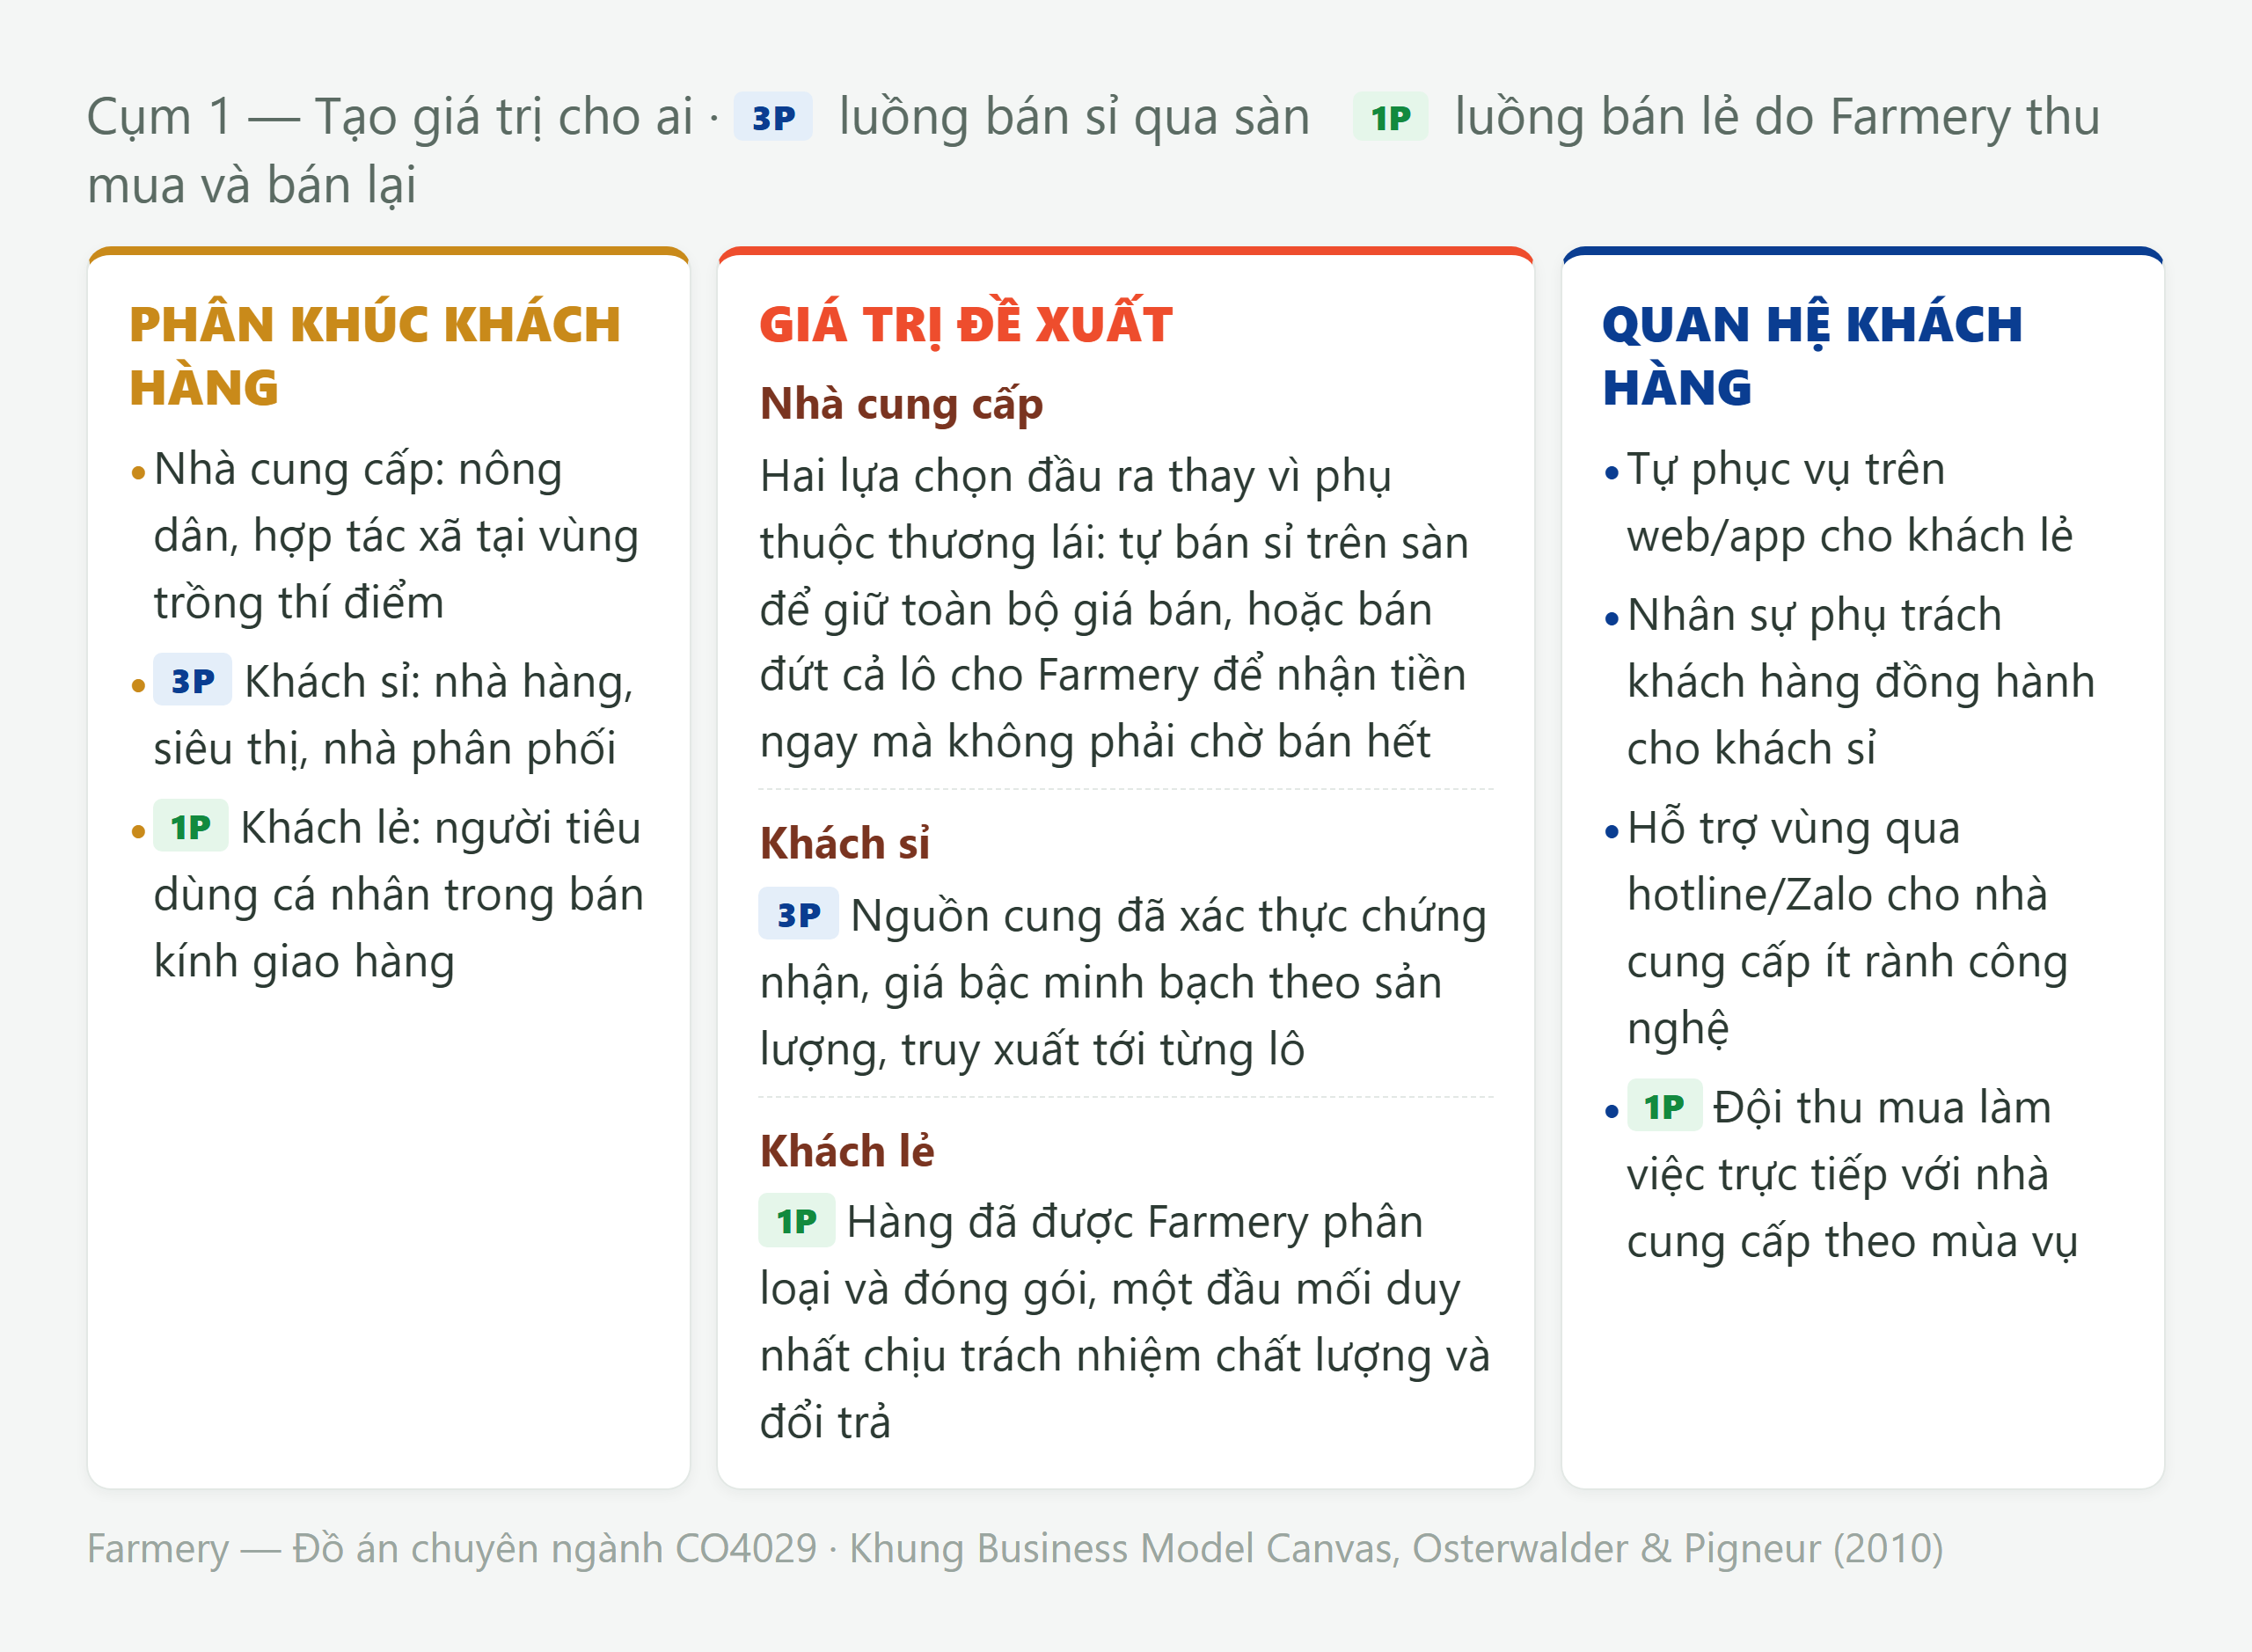
\includegraphics[width=\textwidth]{image/comparison/bmc-cum1.png}
\caption{Business Model Canvas --- cụm tạo giá trị cho ai}
\label{fig:bmc-cum1}
\end{figure}

\begin{figure}[H]
\centering
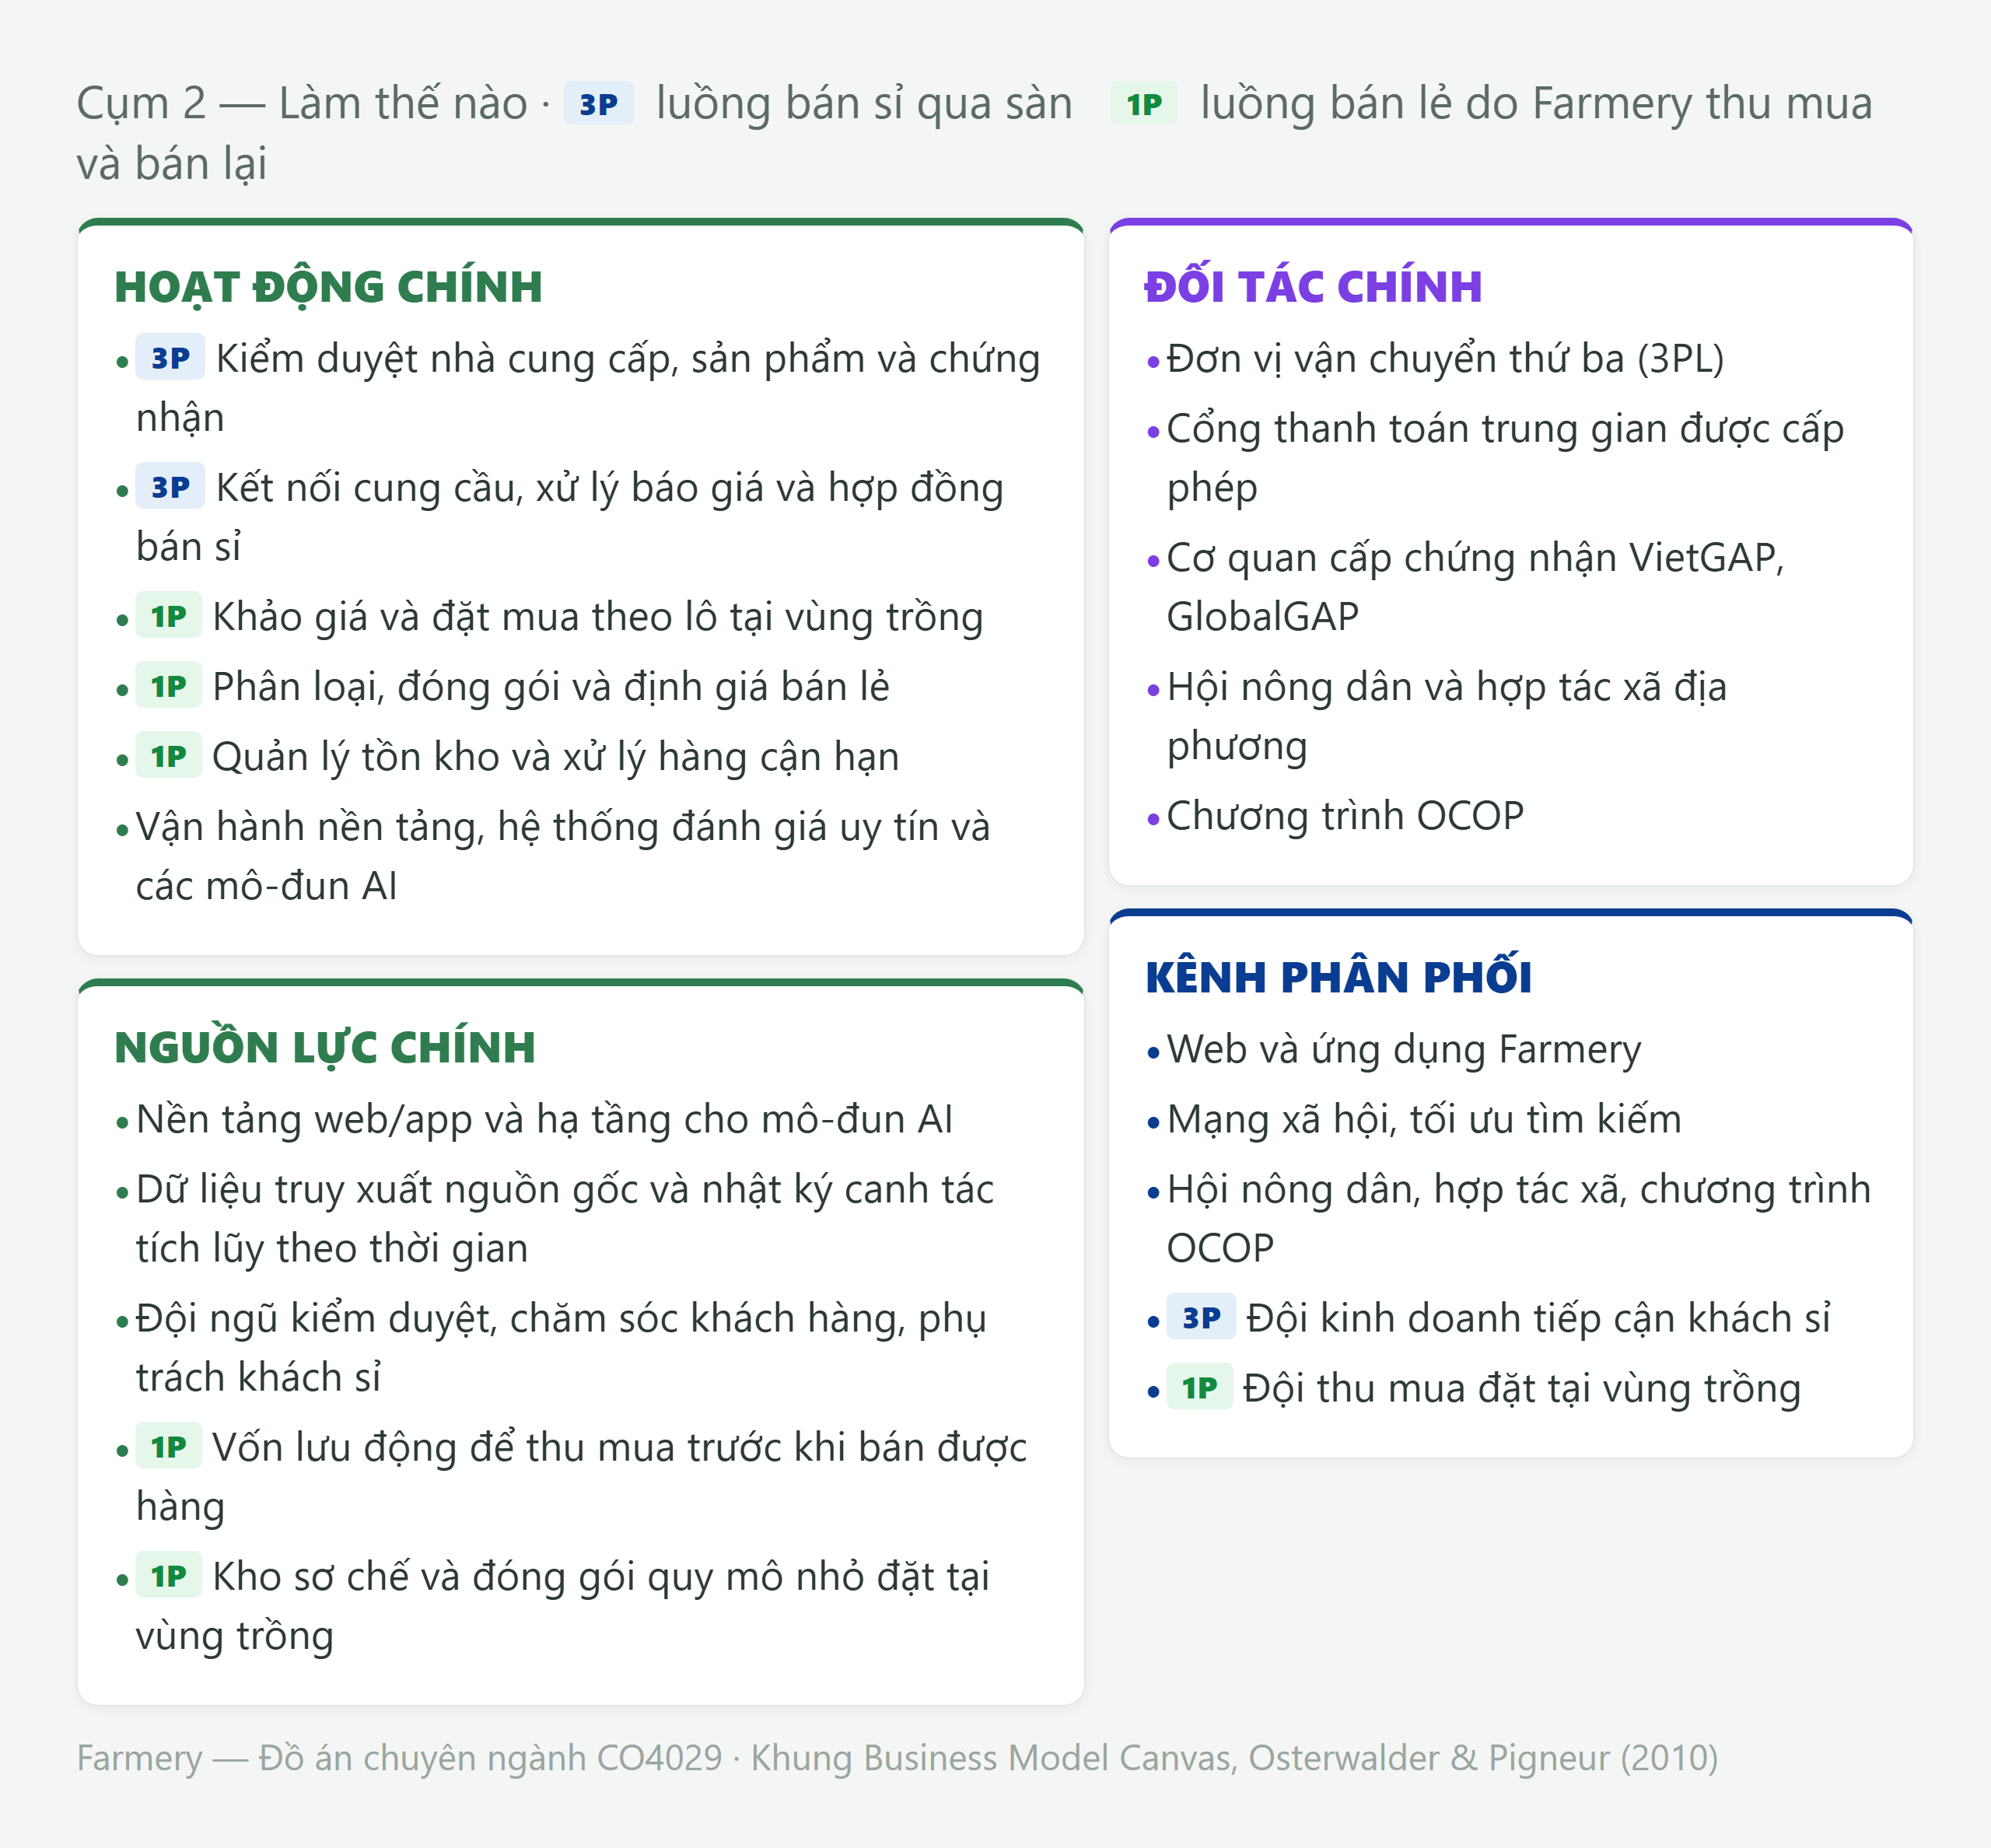
\includegraphics[width=\textwidth]{image/comparison/bmc-cum2.png}
\caption{Business Model Canvas --- cụm cách thức thực hiện}
\label{fig:bmc-cum2}
\end{figure}

\begin{figure}[H]
\centering
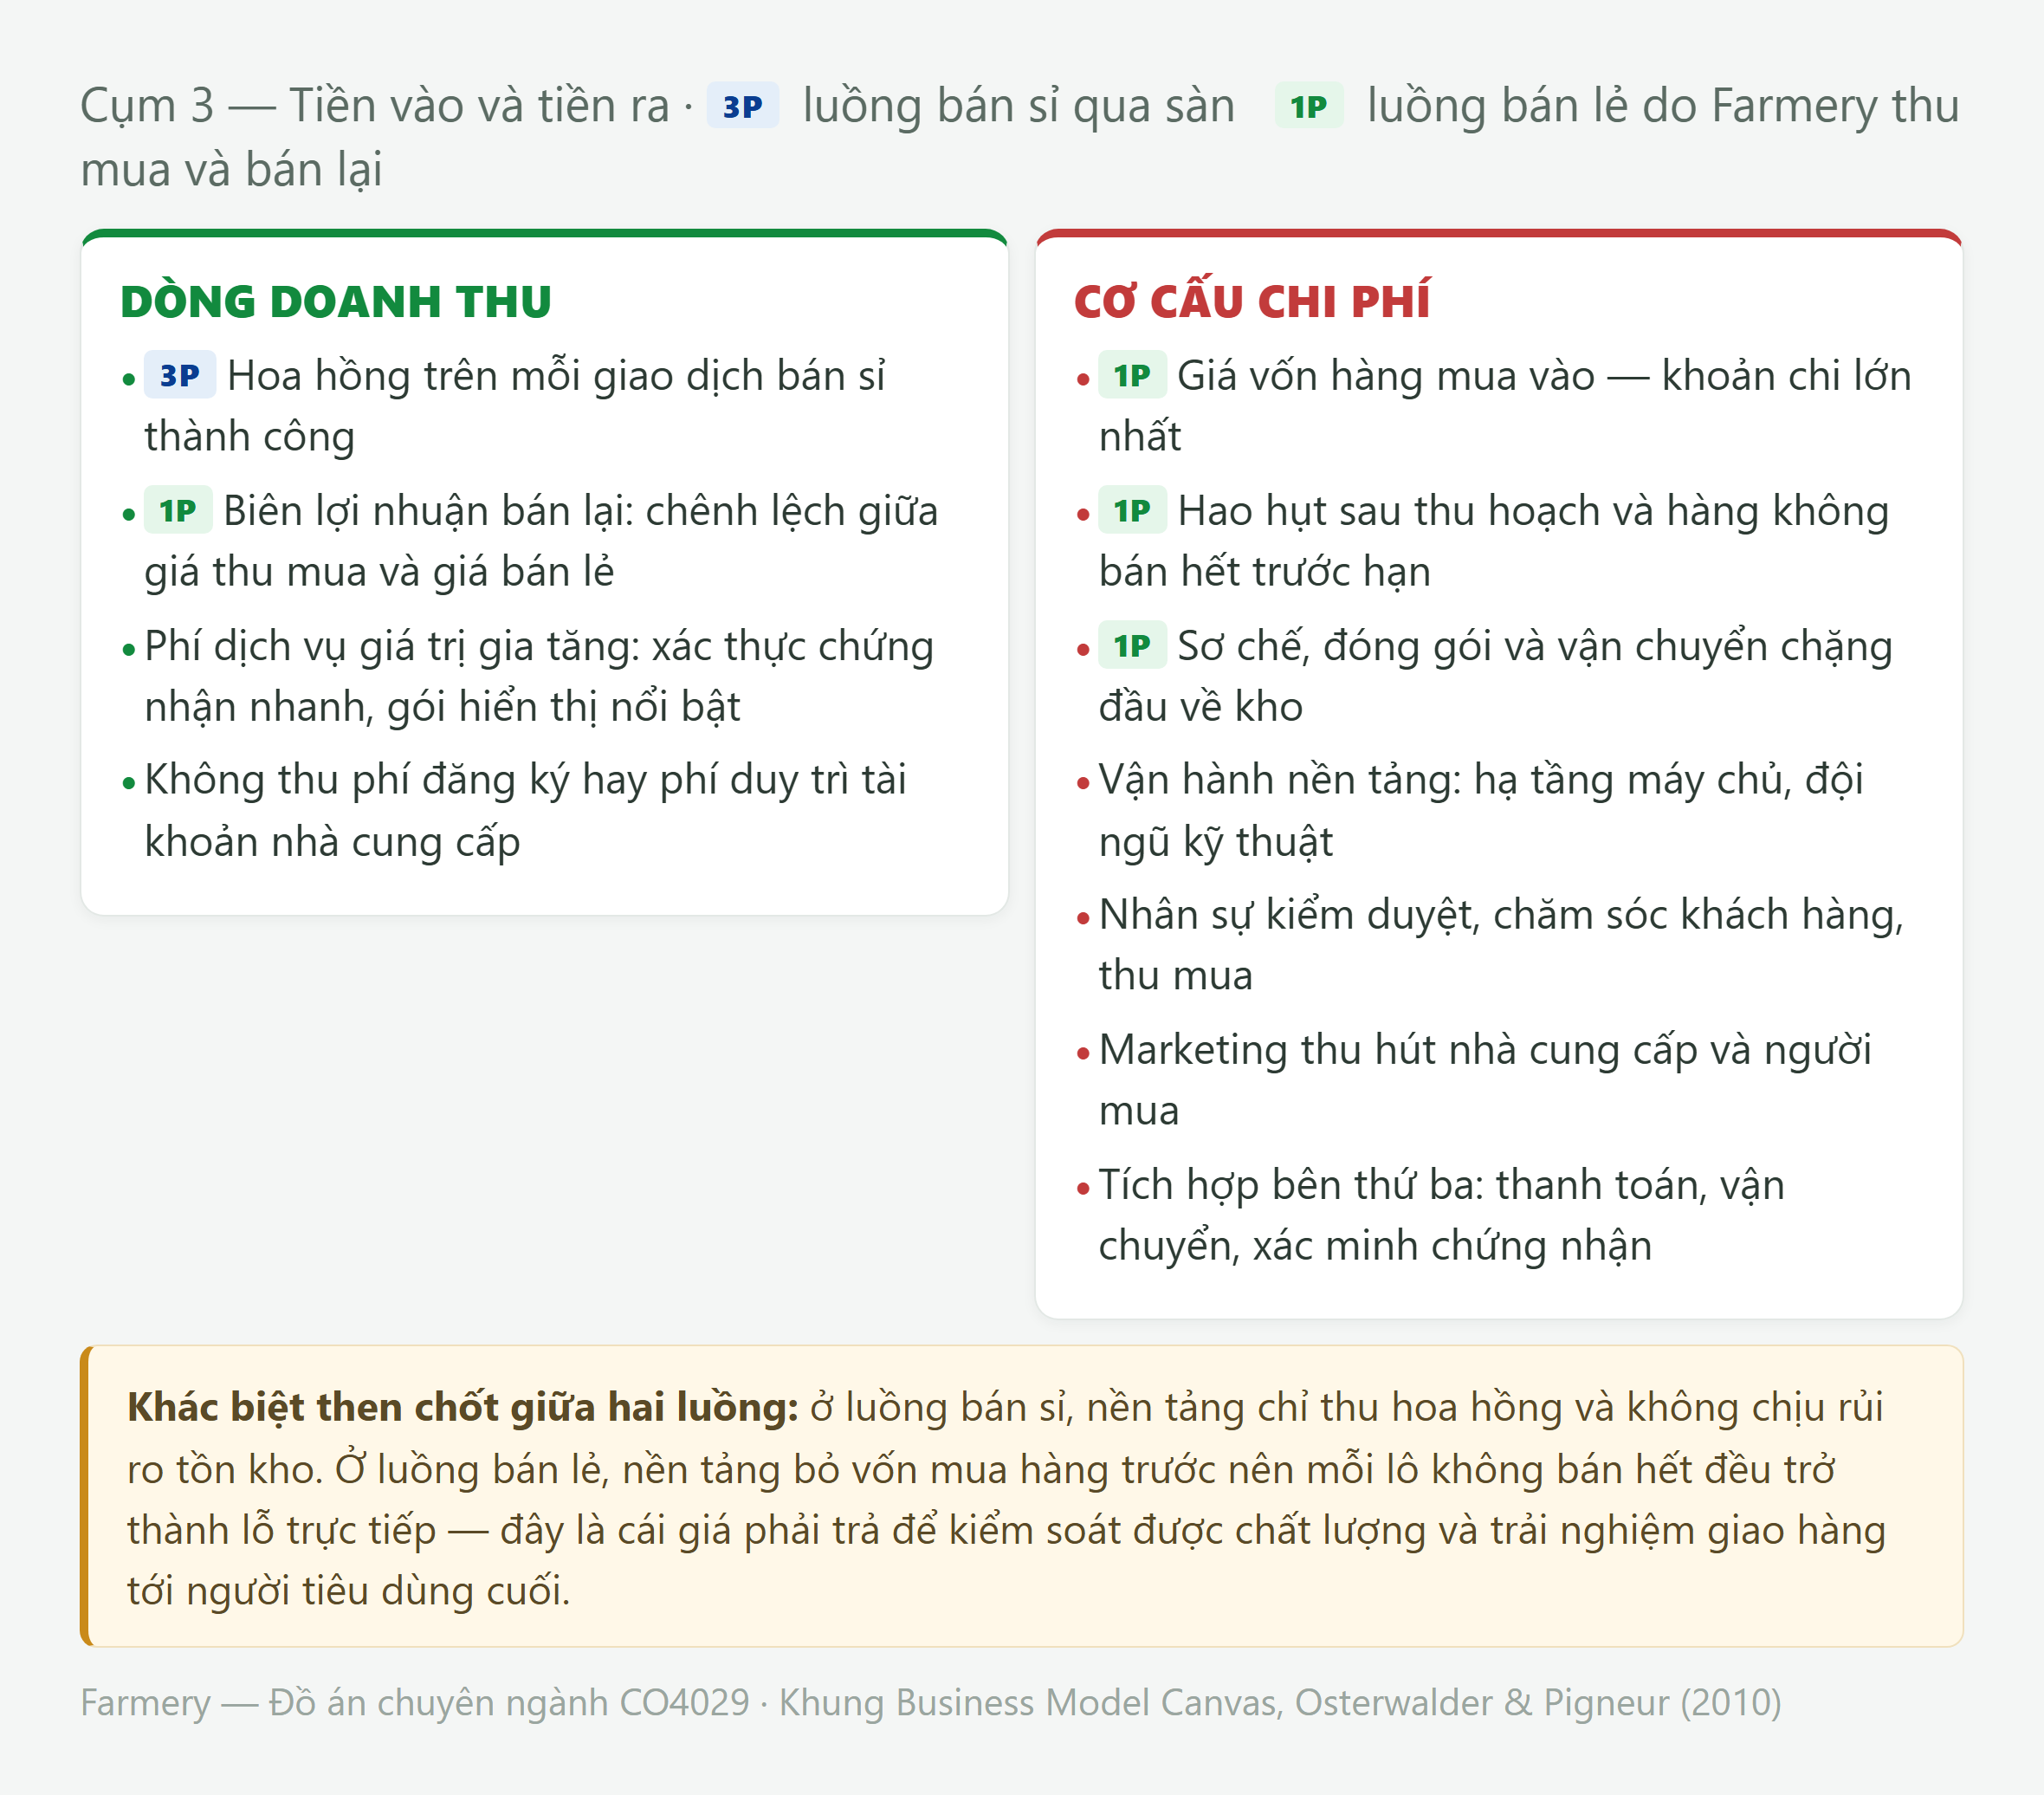
\includegraphics[width=\textwidth]{image/comparison/bmc-cum3.png}
\caption{Business Model Canvas --- cụm dòng tiền vào và ra}
\label{fig:bmc-cum3}
\end{figure}

\noindent\textbf{Các dòng doanh thu.} Ngoài hoa hồng bán sỉ và biên lợi nhuận bán lẻ đã nêu, nền tảng thu thêm phí dịch vụ giá trị gia tăng gồm xác thực chứng nhận nhanh và \emph{gói hiển thị nổi bật}. Cần phân biệt gói hiển thị nổi bật với cơ chế \emph{ưu tiên hiển thị theo uy tín} tại mục~\ref{subsec:danhgianghiepvu}: cơ chế theo uy tín là quyền lợi miễn phí, tự động dành cho nhà cung cấp đạt ngưỡng điểm quy định, còn gói nổi bật là dịch vụ trả phí --- chỉ nhà cung cấp đã đạt cùng ngưỡng uy tín đó mới đủ điều kiện mua, và vị trí mua được gắn nhãn ``Tài trợ'' để tách bạch với kết quả tìm kiếm tự nhiên, tránh làm sai lệch tín hiệu chất lượng mà hệ thống uy tín tạo ra (liên hệ mục~\ref{subsec:reputation}). Nền tảng chủ động không thu phí đăng ký hoặc phí duy trì tài khoản đối với nhà cung cấp, nhằm giảm rào cản gia nhập cho nhóm nông dân và hợp tác xã vốn đã hạn chế về nguồn lực (mục~\ref{sec:doituongnguoidung}) --- chi tiết mức phí cụ thể và các điều khoản liên quan được quy định tại Phụ lục D (Điều khoản dịch vụ).


\subsection{Quy trình nghiệp vụ và quy tắc nghiệp vụ}
\label{sec:quytrinhnghiepvu}

Mỗi quy trình dưới đây được trình bày theo các bước tuần tự, có ghi rõ tác nhân thực hiện, điều kiện chuyển bước (quy tắc nghiệp vụ) và các trường hợp ngoại lệ. Lưu đồ minh họa cho từng quy trình được trình bày tại mục~\ref{subsec:mohinhquytrinh}.

\subsubsection*{Đăng ký và xác thực nhà cung cấp, kiểm duyệt chứng nhận}
\begin{enumerate}
    \item Nhà cung cấp (nông dân hoặc hợp tác xã) đăng ký tài khoản, nhập thông tin định danh (căn cước công dân hoặc mã số thuế đối với hợp tác xã) và thông tin trang trại, vùng canh tác.
    \item Hệ thống gửi mã xác thực (OTP) qua số điện thoại hoặc email; nếu nhập sai quá 5 lần, tài khoản bị khóa tạm thời trong 30 phút.
    \item Nhà cung cấp thực hiện xác minh danh tính điện tử (eKYC --- FR1.4): tải ảnh chụp giấy tờ định danh và ảnh chân dung để hệ thống đối chiếu; kết quả được ghi vào trạng thái eKYC của gian hàng.
    \item Nhà cung cấp tải lên giấy chứng nhận VietGAP, GlobalGAP, hữu cơ (organic), OCOP hoặc HACCP (nếu có), kèm mã số chứng nhận, cơ quan cấp và ngày hết hạn.
    \item Bộ phận kiểm duyệt đối chiếu thông tin chứng nhận với dữ liệu của cơ quan cấp (nếu có kết nối) hoặc xác minh thủ công.
    \item Hệ thống ghi nhận kết quả: nếu eKYC đạt, tài khoản chuyển trạng thái ``Đã xác thực'' và được kích hoạt quyền đăng bán, đồng thời nhãn chứng nhận tương ứng (nếu chứng nhận cũng được duyệt) hiển thị công khai; nếu không đạt ở bước nào, hệ thống gửi thông báo lý do và hướng dẫn bổ sung cho bước đó.
\end{enumerate}

\noindent\textbf{Ngoại lệ:}
\begin{itemize}
    \item Chứng nhận còn hiệu lực dưới 30 ngày: hệ thống tự động nhắc nhà cung cấp gia hạn; nếu hết hạn mà chưa gia hạn, nhãn chứng nhận trên sản phẩm liên quan tự động bị ẩn cho đến khi cập nhật (sản phẩm không bị gỡ bỏ).
    \item Phát hiện chứng nhận giả mạo qua xác minh hoặc khiếu nại: tài khoản bị khóa vĩnh viễn, ghi vào danh sách vi phạm, không được phép đăng ký lại bằng cùng thông tin định danh.
\end{itemize}

\subsubsection*{Đăng và kiểm duyệt sản phẩm, sinh mã QR truy xuất}
\begin{enumerate}
    \item Nhà cung cấp đã xác thực tạo sản phẩm mới với đầy đủ thông tin: tên, mô tả, hình ảnh, đơn vị tính, giá bán lẻ, giá bán sỉ theo bậc (nếu có), sản lượng và ngày dự kiến thu hoạch.
    \item Nhà cung cấp ghi nhật ký canh tác theo từng giai đoạn (gieo trồng, chăm sóc, thu hoạch), mỗi lần ghi gồm ngày tháng, hoạt động và hình ảnh minh chứng nếu có; các bản ghi được gắn với một lô sản phẩm (batch) cụ thể.
    \item Hệ thống kiểm duyệt tự động sơ bộ: kiểm tra hình ảnh không trùng lặp, mô tả không chứa từ khóa cấm, giá không bất thường so với mặt bằng chung của danh mục.
    \item Bộ phận kiểm duyệt thực hiện kiểm tra thủ công lần cuối đối với sản phẩm mới hoặc nhà cung cấp chưa có lịch sử giao dịch; nhà cung cấp có uy tín lâu năm có thể áp dụng cơ chế hậu kiểm để rút ngắn thời gian chờ duyệt.
    \item Hệ thống sinh mã QR truy xuất duy nhất cho từng lô sản phẩm, liên kết tới trang truy xuất công khai gồm hồ sơ nhà cung cấp, chứng nhận, nhật ký canh tác và các mốc vận chuyển liên quan.
\end{enumerate}

\noindent\textbf{Điều kiện:} sản phẩm chỉ được duyệt và hiển thị công khai khi có tối thiểu một bản ghi nhật ký canh tác gần nhất và hình ảnh sản phẩm thực tế.

\noindent\textbf{Quy tắc bảo đảm sản phẩm đăng bán đúng là nông sản.} Vì nền tảng chuyên biệt cho nông sản chứ không phải sàn tổng hợp, việc nhà cung cấp đăng nhầm hoặc cố tình đăng sai loại hàng sẽ làm hỏng chính giá trị mà nền tảng cam kết. Hệ thống kiểm soát điều này bằng bốn lớp:

\begin{enumerate}
    \item[\textbf{L1.}] \textbf{Danh mục đóng.} Sản phẩm bắt buộc gắn vào một danh mục lá trong cây danh mục nông sản do quản trị viên định nghĩa sẵn theo phạm vi tại mục~\ref{subsec:dinhnghianongsan}; nhà cung cấp không được tự tạo danh mục mới. Mỗi danh mục lá quy định sẵn tập đơn vị tính hợp lệ và các trường bắt buộc kèm theo (ngày thu hoạch, hạn bảo quản, vùng trồng), nên hàng không phải nông sản sẽ không tìm được chỗ để khai báo hợp lệ.
    \item[\textbf{L2.}] \textbf{Danh sách loại trừ.} Nền tảng công bố công khai danh sách nhóm hàng không được đăng --- thủy sản sống, thịt tươi, động vật sống, thực phẩm chức năng, thuốc bảo vệ thực vật, vật tư nông nghiệp và mọi hàng hóa phi thực phẩm --- hiển thị ngay tại biểu mẫu đăng sản phẩm để giảm lỗi do hiểu nhầm.
    \item[\textbf{L3.}] \textbf{Kiểm duyệt trước khi hiển thị.} Hệ thống kiểm tra tự động sơ bộ (ảnh trùng lặp, từ khóa cấm, giá lệch bất thường so với mặt bằng danh mục, dấu hiệu sai danh mục), sau đó bộ phận kiểm duyệt kiểm tra thủ công. Với nhóm chế biến sâu, hồ sơ tự công bố sản phẩm là điều kiện bắt buộc để được duyệt.
    \item[\textbf{L4.}] \textbf{Hậu kiểm bằng phản hồi cộng đồng.} Người mua có thể báo cáo sản phẩm sai danh mục hoặc không phải nông sản ngay tại trang sản phẩm; báo cáo được đưa vào hàng đợi xử lý của quản trị viên kiểm duyệt.
\end{enumerate}

\noindent\textbf{Chế tài khi vi phạm} được áp dụng theo ba mức tăng dần: lần đầu ẩn sản phẩm và yêu cầu nhà cung cấp phân loại lại; tái phạm thì cảnh cáo và trừ điểm uy tín (mục~\ref{subsec:danhgianghiepvu}); cố tình đăng hàng thuộc danh sách loại trừ hoặc tái phạm nhiều lần thì khóa quyền đăng bán.

\noindent\textbf{Ngoại lệ:}
\begin{itemize}
    \item Thay đổi thông tin trọng yếu sau khi đã duyệt (giá thay đổi vượt 20\% hoặc mô tả chất lượng thay đổi): sản phẩm chuyển về trạng thái chờ duyệt lại.
    \item Thay đổi nhỏ (còn hàng/hết hàng): không yêu cầu duyệt lại.
\end{itemize}

\subsubsection*{Quy trình thu mua vào kho của nền tảng}

Quy trình này đứng trước quy trình bán lẻ và là điểm khác biệt căn bản so với một sàn thuần trung gian.

\begin{enumerate}
    \item Nhà cung cấp công bố lô hàng sắp thu hoạch kèm sản lượng dự kiến, ngày thu hoạch và giá chào.
    \item Bộ phận thu mua đối chiếu các chào hàng cùng loại trong kỳ, tham khảo dự báo giá (mục~\ref{sec:thietkeAI}) và tồn kho hiện có để quyết định mua lô nào, số lượng bao nhiêu.
    \item Hai bên thống nhất giá và thời điểm giao; hệ thống sinh đơn thu mua và thông báo cho nhà cung cấp.
    \item Nhà cung cấp giao hàng về kho sơ chế tại vùng trồng; bộ phận thu mua kiểm tra chất lượng thực tế và nhập kho theo lô, kế thừa nguyên vẹn nhật ký canh tác và mã QR truy xuất của lô đó.
    \item Hệ thống thanh toán cho nhà cung cấp theo sản lượng đã nghiệm thu --- nhà cung cấp nhận tiền tại bước này, không phải chờ hàng bán được.
    \item Bộ phận thu mua đặt giá bán lẻ dựa trên giá vốn, tỷ lệ hao hụt dự kiến và mặt bằng giá thị trường, sau đó mở bán trên gian hàng của nền tảng.
\end{enumerate}

\noindent\textbf{Ngoại lệ:}
\begin{itemize}
    \item Chất lượng thực tế không đạt so với mô tả: bộ phận thu mua có quyền từ chối nhận hoặc nhận với giá điều chỉnh đã thống nhất lại; trường hợp lệch nghiêm trọng được ghi vào lịch sử uy tín của nhà cung cấp.
    \item Lô đã nhập kho tồn quá lâu hoặc cận hạn: hệ thống cảnh báo để bộ phận thu mua chủ động giảm giá xả hàng, chấp nhận biên lợi nhuận thấp thay vì mất trắng.
    \item Lô đang rao bán sỉ sắp hết hạn bảo quản mà chưa có người mua: hệ thống đề xuất để nền tảng thu mua lại với giá chiết khấu, chuyển sang kênh bán lẻ.
\end{itemize}

\subsubsection*{Quy trình bán lẻ}

Ở luồng này, bên bán là chính nền tảng: hàng đã thuộc sở hữu của Farmery từ quy trình thu mua ở trên.

\begin{enumerate}
    \item Khách lẻ tìm kiếm và lọc sản phẩm theo danh mục, vùng trồng, chứng nhận hoặc mức giá.
    \item Khách lẻ xem chi tiết sản phẩm, có thể tra cứu trang truy xuất nguồn gốc --- vẫn dẫn tới nhật ký canh tác của nhà cung cấp gốc --- trước khi quyết định mua.
    \item Khách lẻ thêm sản phẩm vào giỏ hàng, số lượng giới hạn theo tồn kho còn lại của lô.
    \item Khách lẻ thanh toán qua ví điện tử, chuyển khoản hoặc thanh toán khi nhận hàng, đồng thời chọn khung giờ giao phù hợp với hàng tươi.
    \item Hệ thống xác nhận đơn hàng và trừ tồn kho của lô tương ứng; thao tác trừ tồn thực hiện trong một giao dịch có khóa để tránh bán vượt khi lô đó đồng thời được giao dịch ở kênh bán sỉ.
    \item Nhân sự tại kho đóng gói theo tiêu chuẩn dành cho hàng dễ hư hỏng và bàn giao cho đơn vị vận chuyển.
    \item Khách lẻ xác nhận đã nhận hàng và có thể đánh giá sản phẩm trong khoảng thời gian quy định.
\end{enumerate}

\noindent\textbf{Ngoại lệ:}
\begin{itemize}
    \item Thanh toán trực tuyến thất bại: đơn hàng giữ trạng thái chờ thanh toán tối đa 15 phút trước khi tự hủy và hoàn lại tồn kho.
    \item Người nhận từ chối nhận hàng khi trả tiền mặt: đơn chuyển trạng thái hoàn hàng; do là hàng tươi, lô trả về được đánh giá lại chất lượng trước khi quyết định bán tiếp hay hủy.
    \item Nhiều đơn đặt cùng lúc vượt tồn kho còn lại: hệ thống ưu tiên đơn xác nhận trước; các đơn còn lại tự động hủy kèm thông báo hết hàng.
    \item Hàng giao không đạt chất lượng: Farmery chịu trách nhiệm đổi trả trực tiếp với khách lẻ, sau đó mới đối chiếu lại với nhà cung cấp gốc nếu nguyên nhân thuộc về khâu cung ứng.
\end{itemize}

\subsubsection*{Đánh giá sản phẩm và nhà cung cấp}
\label{subsec:danhgianghiepvu}

\begin{enumerate}
    \item Người mua đã xác nhận nhận hàng (bước cuối quy trình bán lẻ ở trên) được quyền gửi đánh giá gồm điểm số (1--5 sao), bình luận và hình ảnh, trong khung thời gian quy định sau khi nhận hàng --- chỉ áp dụng cho đơn hàng đã xác nhận (verified purchase), không cho phép đánh giá khi chưa mua.
    \item Hệ thống kiểm duyệt tự động sơ bộ (từ khóa cấm, liên kết đáng ngờ) kết hợp các luật ngưỡng giám sát bất thường (Chương~\ref{chap:coso}) để phát hiện đánh giá giả hoặc thao túng uy tín.
    \item Đánh giá không bị nghi ngờ được công khai ngay; đánh giá bị nghi ngờ chuyển cho quản trị viên xem xét thủ công trước khi công khai hoặc ẩn.
    \item Hệ thống cập nhật điểm uy tín tổng hợp của nhà cung cấp --- trung bình có trọng số theo thời gian và số lượng đơn, không tính các đánh giá bị ẩn.
    \item Nhà cung cấp có thể phản hồi công khai một lần dưới mỗi đánh giá.
\end{enumerate}

\noindent\textbf{Thang đo điểm uy tín (đo lường):} điểm uy tín tổng hợp được chuẩn hóa về thang 0--100 (không dùng trực tiếp thang 1--5 sao của từng đánh giá đơn lẻ), tính bằng trung bình có trọng số của điểm sao các đánh giá hợp lệ trong 6 tháng gần nhất, trong đó đánh giá gần đây và đánh giá gắn với đơn hàng giá trị lớn hơn được gán trọng số cao hơn đánh giá cũ/đơn giá trị nhỏ. Ngưỡng áp dụng cơ chế hậu kiểm nhanh và ưu tiên hiển thị được đặt ở mức từ 80/100 trở lên.

\noindent\textbf{Căn cứ:} thang 0--100 giúp phân biệt mức độ uy tín rõ ràng hơn thang 1--5 sao, vốn dễ bị dồn cụm ở mức 4--5 sao do tâm lý người mua ngại để lại đánh giá tiêu cực \parencite{springer_article}; trọng số theo thời gian đảm bảo điểm phản ánh chất lượng gần đây thay vì phụ thuộc mãi vào lịch sử cũ (một nhà cung cấp từng tốt nhưng gần đây sa sút chất lượng không nên tiếp tục hưởng cơ chế ưu tiên); ngưỡng 80/100 được đặt ở mức cao vì cơ chế hậu kiểm nhanh làm giảm bớt kiểm soát trước khi đăng bán, nên chỉ nên áp dụng cho nhà cung cấp thực sự đáng tin cậy, nhằm hạn chế rủi ro bị lợi dụng.

\noindent\textbf{Điều kiện:} nhà cung cấp đạt điểm uy tín từ ngưỡng quy định trở lên được áp dụng cơ chế hậu kiểm nhanh khi đăng sản phẩm mới (đã nêu tại mục~\ref{sec:quytrinhnghiepvu}, Đăng và kiểm duyệt sản phẩm) và được ưu tiên hiển thị trong kết quả tìm kiếm.

\noindent\textbf{Ngoại lệ:}
\begin{itemize}
    \item Đánh giá bị từ chối sau kiểm duyệt thủ công: ẩn khỏi trang sản phẩm, thông báo lý do cho người mua, không tính vào điểm uy tín.
    \item Nhà cung cấp bị phát hiện thao túng đánh giá (mua đánh giá ảo, trả đũa khách hàng qua kênh ngoài hệ thống): xử lý theo quy trình vi phạm tại mục~\ref{sec:quytrinhnghiepvu} (Quản trị hệ thống).
\end{itemize}

\subsubsection*{Quy trình bán sỉ (B2B)}
\begin{enumerate}
    \item Nhà cung cấp công bố bảng giá bán sỉ theo bậc số lượng, số lượng tối thiểu (MOQ) và lịch giao dự kiến cho từng sản phẩm/lô hàng.
    \item Doanh nghiệp thu mua xem bảng giá công khai, gửi yêu cầu báo giá (RFQ) tham chiếu bảng giá hoặc yêu cầu tùy chỉnh nếu nhu cầu khác chuẩn (sản phẩm, số lượng, tiêu chuẩn chất lượng, lịch giao).
    \item Hệ thống kiểm tra số lượng yêu cầu có đạt MOQ của nhà cung cấp hay không; nếu chưa đạt, hệ thống gợi ý gộp đơn với doanh nghiệp khác cùng khu vực hoặc chuyển hướng sang kênh bán lẻ.
    \item Nhà cung cấp xác nhận hoặc điều chỉnh báo giá theo bậc, thời gian có thể đáp ứng và điều kiện thanh toán.
    \item Hai bên thương lượng qua hệ thống nhắn tin nội bộ cho đến khi thống nhất số lượng, đơn giá và lịch giao.
    \item Hệ thống sinh hợp đồng điện tử từ mẫu chuẩn, điền đầy đủ các điều khoản đã thống nhất, bao gồm điều khoản phạt vi phạm và điều khoản thanh toán theo từng đợt giao.
    \item Hai bên ký xác nhận hợp đồng bằng chữ ký điện tử hoặc mã xác nhận trong hệ thống.
    \item Nếu hợp đồng thuộc diện áp dụng ký quỹ trung gian (giá trị vượt ngưỡng quy định --- FR7.3), bên mua nộp tiền của đợt giao vào tài khoản ký quỹ tại cổng thanh toán trung gian trước khi nhà cung cấp giao hàng; hệ thống ghi nhận trạng thái ``đã ký quỹ'' và thông báo cho nhà cung cấp, bản thân nền tảng không giữ tiền.
    \item Nhà cung cấp giao hàng theo từng đợt theo lịch đã ký; mỗi đợt giao, hệ thống sinh hóa đơn tương ứng cho đợt đó.
    \item Doanh nghiệp thu mua xác nhận nhận hàng và chất lượng từng đợt, sau đó thanh toán cho đợt giao đó; với hợp đồng có ký quỹ, hệ thống ra lệnh cho cổng thanh toán trung gian giải ngân khoản đã giữ cho nhà cung cấp ngay tại bước xác nhận này.
    \item Nhà cung cấp theo dõi doanh thu và lịch sử bán sỉ theo hợp đồng đã hoàn tất trên trang quản lý của mình.
\end{enumerate}

\noindent\textbf{Ngoại lệ:}
\begin{itemize}
    \item Nhà cung cấp không giao đủ số lượng/đúng lịch một đợt giao: áp dụng điều khoản phạt trong hợp đồng, ghi nhận vào lịch sử uy tín của nhà cung cấp.
    \item Doanh nghiệp thu mua chậm thanh toán một đợt giao: hệ thống nhắc nhở tự động, có thể tạm khóa quyền đặt RFQ mới cho đến khi hoàn tất thanh toán.
    \item Một trong hai bên muốn hủy hợp đồng giữa kỳ: xử lý theo điều khoản hủy đã ký kết từ đầu.
    \item Phát sinh tranh chấp về đợt giao đã ký quỹ: khoản ký quỹ được giữ nguyên tại cổng thanh toán trung gian, không giải ngân cũng không hoàn trả, cho đến khi khiếu nại được xử lý xong theo quy trình tại mục~\ref{sec:quytrinhnghiepvu} (Quản lý tồn kho, vận chuyển hàng dễ hư hỏng và xử lý khiếu nại).
\end{itemize}

\subsubsection*{Quản lý tồn kho, vận chuyển hàng dễ hư hỏng và xử lý khiếu nại}
Trước khi vận chuyển, tồn kho theo lô của nhà cung cấp (đã tạo tại mục~\ref{sec:quytrinhnghiepvu}, Đăng và kiểm duyệt sản phẩm) được quản lý theo nguyên tắc FEFO (mục~\ref{subsec:khobai}): hệ thống ưu tiên gợi ý bán/xuất trước các lô sắp hết hạn hoặc gần ngày thu hoạch nhất, cảnh báo cho nhà cung cấp khi tồn kho một lô xuống dưới ngưỡng hoặc sắp hết hạn mà chưa bán hết, và đồng bộ số lượng còn lại giữa kênh bán lẻ (mục~\ref{sec:quytrinhnghiepvu}, Quy trình bán lẻ) và bán sỉ (mục~\ref{sec:quytrinhnghiepvu}, Quy trình bán sỉ) trên cùng một lô để tránh bán trùng vượt sản lượng thực có. Farmery không vận hành kho trung chuyển quy mô lớn (mục~\ref{subsec:khobai}): ở luồng bán sỉ, nhà cung cấp tự bảo quản và đóng gói hàng tại chỗ trước khi bàn giao cho đơn vị vận chuyển thứ ba; ở luồng bán lẻ, hàng đã thu mua được sơ chế và đóng gói tại kho nhỏ đặt ngay tại vùng trồng.

\begin{enumerate}
    \item Nhà cung cấp đóng gói theo hướng dẫn bảo quản riêng cho từng nhóm nông sản (nhiệt độ, độ ẩm, vật liệu chống dập) do hệ thống gợi ý theo danh mục sản phẩm.
    \item Hệ thống ưu tiên lựa chọn phương thức vận chuyển có hỗ trợ bảo quản lạnh hoặc thời gian giao nhanh đối với các danh mục được đánh dấu dễ hư hỏng; đơn hàng có thời gian giao vượt ngưỡng an toàn sẽ được cảnh báo trước khi khách xác nhận đặt hàng.
    \item Đơn vị vận chuyển cập nhật trạng thái đơn hàng theo thời gian thực trong suốt quá trình giao nhận.
    \item Người nhận kiểm tra hàng ngay khi nhận; nếu phát hiện hư hỏng, gửi khiếu nại trong khung thời gian quy định kèm hình ảnh hoặc video minh chứng.
    \item Hệ thống phân loại khiếu nại theo nguyên nhân khả năng (đóng gói/chất lượng từ nhà cung cấp, lỗi vận chuyển, hoặc bảo quản sai từ phía người nhận).
    \item Bộ phận phụ trách ra quyết định xử lý: hoàn tiền toàn phần, hoàn tiền một phần, đổi lô hàng mới, hoặc từ chối khiếu nại nếu bằng chứng không đầy đủ.
\end{enumerate}

\noindent\textbf{Ngoại lệ:}
\begin{itemize}
    \item Khiếu nại lặp lại nhiều lần từ cùng một nhà cung cấp trong thời gian ngắn: tự động gắn cờ cảnh báo, tạm hạ mức ưu tiên hiển thị sản phẩm cho đến khi được rà soát.
    \item Khiếu nại có dấu hiệu bất thường từ phía người mua: chuyển bộ phận quản trị xem xét thủ công trước khi hoàn tiền.
\end{itemize}

\subsubsection*{Quản trị hệ thống}
\begin{enumerate}
    \item Quản trị viên thực hiện kiểm duyệt định kỳ hồ sơ nhà cung cấp mới, sản phẩm mới hoặc có thay đổi trọng yếu, và các chứng nhận sắp hết hạn.
    \item Quản trị viên giám sát các cảnh báo tự động từ hệ thống, bao gồm tỷ lệ khiếu nại bất thường và các dấu hiệu giao dịch đáng ngờ do luật ngưỡng cấu hình sẵn kích hoạt (Chương~\ref{chap:coso}).
    \item Vi phạm được xử lý theo quy trình phân cấp từ nhắc nhở, cảnh cáo công khai, tạm khóa cho đến khóa vĩnh viễn tài khoản, tùy theo mức độ và số lần vi phạm, có lưu vết đầy đủ lý do và quyết định.
    \item Quản trị viên truy xuất báo cáo thống kê định kỳ để hỗ trợ ra quyết định vận hành và báo cáo cho các bên liên quan.
\end{enumerate}

Ngoại lệ: khi phát hiện vi phạm nghiêm trọng như giả mạo chứng nhận hoặc gian lận, tài khoản bị khóa ngay lập tức mà không qua các bước nhắc nhở trung gian, đồng thời toàn bộ đơn hàng đang xử lý của tài khoản đó được rà soát để bảo vệ quyền lợi của khách hàng đã đặt trước.

\subsection{Chính sách, pháp lý và đạo đức}
\label{subsec:chinhsach}

Các chính sách dưới đây chi phối cách sàn vận hành và được cụ thể hóa trong Điều khoản dịch vụ (Phụ lục D):
\begin{itemize}
    \item \textbf{Tuân thủ pháp luật:} hoạt động thương mại điện tử theo Nghị định 52/2013/NĐ-CP và 85/2021/NĐ-CP; bảo vệ dữ liệu cá nhân theo Nghị định 13/2023/NĐ-CP; hóa đơn điện tử theo Thông tư 78/2021/TT-BTC (NFR8).
    \item \textbf{Không trực tiếp giữ tiền của người dùng:} thanh toán và ký quỹ escrow được xử lý qua cổng thanh toán trung gian được cấp phép; Farmery chỉ ghi nhận trạng thái và ra lệnh giải ngân (FR7.3, NFR3.4).
    \item \textbf{Minh bạch và công bằng trong xếp hạng:} ưu tiên hiển thị theo uy tín là quyền lợi miễn phí; gói hiển thị nổi bật trả phí phải gắn nhãn ``Tài trợ'' để không làm sai lệch tín hiệu chất lượng (mục~\ref{sec:businessmodelcanvas}).
    \item \textbf{Chống gian lận và thao túng:} chỉ người đã mua mới được đánh giá; đánh giá nghi vấn được kiểm duyệt thủ công; vi phạm xử lý phân cấp, vi phạm nghiêm trọng (giả mạo chứng nhận, gian lận) bị khóa ngay và có lưu vết quyết định.
    \item \textbf{Toàn vẹn dữ liệu truy xuất:} nhật ký canh tác và chứng nhận đã công khai không được sửa trực tiếp, mọi đính chính phải tạo bản ghi mới (NFR9.1).
    \item \textbf{Sử dụng dữ liệu cho AI:} dữ liệu do nhà cung cấp cung cấp thuộc quyền sở hữu của nhà cung cấp; Farmery chỉ dùng để vận hành nền tảng và huấn luyện mô-đun AI, ở dạng ẩn danh/tổng hợp khi không cần gắn với danh tính (Phụ lục D, Điều 9).
\end{itemize}

\section{Mô tả hệ thống}
\label{sec:motahethong}

\subsection{Tổng quan về hệ thống}
\label{sec:luongvanhanh}

\subsubsection*{Farmery là gì}

Farmery là nền tảng thương mại điện tử chuyên biệt cho nông sản, vận hành đồng thời hai luồng đã mô tả tại mục~\ref{sec:businessmodelcanvas}: một sàn bán sỉ nơi nông dân và hợp tác xã tự bán cho doanh nghiệp thu mua, và một gian hàng bán lẻ nơi chính nền tảng thu mua hàng rồi bán lại cho người tiêu dùng. Điểm xuyên suốt cả hai luồng là mọi sản phẩm đều gắn với một lô cụ thể có nhật ký canh tác và chứng nhận đã qua kiểm duyệt, tra cứu được bằng mã QR công khai.

Để tránh hiểu nhầm về phạm vi, cần nói rõ Farmery \emph{không phải} những thứ sau:
\begin{itemize}
    \item \textbf{Không phải sàn thương mại điện tử tổng hợp:} danh mục hàng hóa giới hạn trong nhóm nông sản đã định nghĩa tại mục~\ref{subsec:dinhnghianongsan}; sản phẩm ngoài nhóm này bị từ chối ngay ở khâu đăng bán.
    \item \textbf{Không phải dịch vụ đi chợ hộ:} nền tảng không nhận mua hộ theo yêu cầu từng khách, mà bán hàng đã thu mua sẵn theo lô.
    \item \textbf{Không tự vận hành hệ thống kho lạnh quy mô lớn:} chỉ duy trì kho sơ chế và đóng gói nhỏ tại vùng trồng phục vụ luồng bán lẻ, phần vận chuyển thuê đơn vị thứ ba (mục~\ref{subsec:khobai}).
\end{itemize}

\subsubsection*{Các phân hệ chức năng}

Nền tảng được tổ chức thành các phân hệ dưới đây, mỗi phân hệ ứng với một nhóm yêu cầu chức năng tại mục~\ref{sec:yeucauchucnang}:
\begin{itemize}
    \item \textbf{Tài khoản và phân quyền} (FR1) --- đăng ký, xác thực, gán vai trò cho cả người dùng ngoài lẫn nhân sự nội bộ.
    \item \textbf{Hồ sơ nhà cung cấp và chứng nhận} (FR2, FR3) --- gian hàng, vùng canh tác, quản lý hiệu lực chứng nhận.
    \item \textbf{Sản phẩm và truy xuất nguồn gốc} (FR4) --- danh mục nông sản, nhật ký canh tác theo lô, sinh mã QR, trang truy xuất công khai.
    \item \textbf{Bán sỉ} (FR6) --- bảng giá bậc, yêu cầu báo giá, hợp đồng và lịch giao theo đợt.
    \item \textbf{Bán lẻ} (FR5) --- gian hàng do nền tảng vận hành, giỏ hàng, đặt hàng và đổi trả.
    \item \textbf{Thu mua và tồn kho} (FR2.3, FR11.2) --- đơn thu mua theo lô, tồn kho theo nguyên tắc xuất trước hàng hết hạn trước, cảnh báo hàng cận hạn.
    \item \textbf{Thanh toán} (FR7) --- kết nối cổng thanh toán, tạm giữ tiền cho đơn sỉ, đối soát.
    \item \textbf{Vận chuyển và khiếu nại} (FR8) --- kết nối đơn vị vận chuyển, theo dõi hành trình, xử lý khiếu nại hàng hư hỏng.
    \item \textbf{Đánh giá và uy tín} (FR9) --- điểm uy tín nhà cung cấp, kiểm soát đánh giá giả.
    \item \textbf{Quản trị} (FR10) --- kiểm duyệt, xử lý vi phạm, báo cáo thống kê.
    \item \textbf{Hỗ trợ AI} (FR12) --- gợi ý sản phẩm, dự báo giá, trợ lý ảo.
\end{itemize}

\subsubsection*{Kênh truy cập}

Người dùng tiếp cận nền tảng qua giao diện web đáp ứng nhiều kích thước màn hình --- lựa chọn này phù hợp với nhóm nông dân và hợp tác xã vốn chủ yếu dùng điện thoại nhưng ngại cài thêm ứng dụng. Riêng trang truy xuất nguồn gốc mở công khai, không yêu cầu đăng nhập, để người mua quét mã QR trên bao bì là xem được ngay. Ứng dụng di động riêng và kênh hỗ trợ qua Zalo nằm ngoài phạm vi đồ án (mục~\ref{sec:phamvi}).

\subsubsection*{Các tác nhân và luồng tương tác}

% TODO: nhóm vẽ sơ đồ ngữ cảnh (context diagram) minh họa nội dung mô tả dưới đây và chèn bằng \includegraphics.
Tổng hợp từ các quy trình nghiệp vụ tại mục~\ref{sec:quytrinhnghiepvu}, các tác nhân tương tác với hệ thống như sau:

\begin{itemize}
    \item \textbf{Nhà cung cấp} --- nông dân, hợp tác xã: đăng ký và xác thực, đăng sản phẩm, ghi nhật ký canh tác, phản hồi yêu cầu báo giá từ khách sỉ, hoặc bán đứt lô hàng cho bộ phận thu mua; giao hàng và nhận thanh toán.
    \item \textbf{Khách sỉ} --- doanh nghiệp thu mua: gửi yêu cầu báo giá, thương lượng và ký hợp đồng với nhà cung cấp qua kênh do hệ thống trung gian hóa, theo dõi tiến độ giao hàng theo từng đợt.
    \item \textbf{Khách lẻ} --- người tiêu dùng cá nhân: tìm kiếm, tra cứu truy xuất, đặt hàng từ gian hàng của nền tảng, nhận hàng và đánh giá. Khách lẻ giao dịch với Farmery chứ không với nhà cung cấp.
    \item \textbf{Bộ phận thu mua:} khảo giá, tạo đơn thu mua theo lô, định giá bán lẻ và theo dõi tồn kho của luồng bán lẻ.
    \item \textbf{Quản trị viên:} kiểm duyệt nhà cung cấp, sản phẩm và chứng nhận; xử lý vi phạm và khiếu nại; truy cập báo cáo thống kê toàn hệ thống.
    \item \textbf{Hệ thống nền tảng:} xác thực OTP, kiểm duyệt tự động sơ bộ, sinh mã QR, phục vụ kết quả từ các mô-đun AI, xử lý thanh toán và điều phối dữ liệu giữa các tác nhân; đồng thời gọi API của các dịch vụ bên thứ ba về thanh toán và vận chuyển.
\end{itemize}

Một nguyên tắc chi phối toàn hệ thống: nền tảng không cho phép bên bán và bên mua giao dịch ngoài tầm kiểm soát của mình. Mọi luồng tiền, dữ liệu chứng nhận và đánh giá đều đi qua hệ thống, vừa để đảm bảo tính minh bạch (liên hệ mục~\ref{subsec:reputation}), vừa để quản trị viên có đủ dữ liệu giám sát và xử lý vi phạm. Ở luồng bán lẻ, nguyên tắc này thể hiện theo cách mạnh hơn: Farmery không đứng giữa mà là một bên trong giao dịch, trực tiếp chịu trách nhiệm chất lượng hàng bán ra trước người tiêu dùng.

\subsubsection*{Các nhóm người dùng}
\label{sec:doituongnguoidung}

Theo mô hình hai luồng tại mục~\ref{sec:businessmodelcanvas}, hệ thống phục vụ năm nhóm người dùng. Nhà cung cấp là nguồn hàng đầu chuỗi và tham gia cả hai luồng; khách sỉ chỉ xuất hiện ở luồng bán sỉ; khách lẻ chỉ xuất hiện ở luồng bán lẻ; bộ phận thu mua và quản trị viên là hai nhóm vận hành nội bộ của nền tảng. Mục này tập trung vào \emph{khó khăn} của từng nhóm --- phần nhu cầu được phát biểu thành user story tại mục~\ref{sec:yeucau} để dẫn thẳng sang yêu cầu hệ thống.

\paragraph*{a) Nhà cung cấp (nông dân, hợp tác xã)}
\begin{itemize}
    \item \textbf{Khó khăn:} hạn chế kỹ năng số và thiết bị (điện thoại thông minh, internet ổn định ở vùng sâu vùng xa); thiếu năng lực tự chụp ảnh, ghi nhật ký canh tác đúng chuẩn, và đặc biệt là không đủ nhân lực để phân loại, đóng gói, xử lý từng đơn lẻ vài ki-lô-gam; e ngại công nghệ và lo sợ bị nền tảng ``thu phí thay thương lái'' mà không mang lại giá tốt hơn thực chất.
    \item \textbf{Vai trò hệ thống (RBAC):} \texttt{seller} --- được gán sau khi hoàn tất xác thực (mục~\ref{sec:luongtiepcan}).
\end{itemize}

\paragraph*{b) Khách sỉ --- doanh nghiệp thu mua (luồng bán sỉ)}
\begin{itemize}
    \item \textbf{Khó khăn:} khó tìm và xác minh nhiều nhà cung cấp nhỏ lẻ phân tán; rủi ro đứt gãy cung ứng khi mất mùa hoặc nhà cung cấp không đáp ứng sản lượng tối thiểu (MOQ); thiếu công cụ quản lý hợp đồng tập trung khi làm việc với nhiều nông dân và hợp tác xã riêng lẻ.
    \item \textbf{Vai trò hệ thống (RBAC):} \texttt{buyer\_wholesale} --- được gán sau khi đội ngũ kinh doanh xác minh hồ sơ doanh nghiệp (mục~\ref{sec:luongtiepcan}).
\end{itemize}

\paragraph*{c) Khách lẻ --- người tiêu dùng cá nhân (luồng bán lẻ)}
\begin{itemize}
    \item \textbf{Khó khăn:} khó phân biệt sản phẩm ``sạch'' thật với sản phẩm gắn mác marketing (do bất cân xứng thông tin --- mục~\ref{subsec:reputation}); lo ngại hàng tươi bị hư hỏng trong vận chuyển; thói quen mua tại chợ và siêu thị truyền thống vẫn phổ biến, đòi hỏi nền tảng phải tạo được lòng tin đủ lớn để thay đổi hành vi.
    \item \textbf{Vai trò hệ thống (RBAC):} \texttt{buyer\_retail} --- được gán ngay sau xác thực OTP (mục~\ref{sec:luongtiepcan}).
\end{itemize}

\paragraph*{d) Bộ phận thu mua và vận hành hàng của Farmery (luồng bán lẻ)}

Đây là nhóm người dùng phát sinh riêng từ luồng bán lẻ: khác với sàn thuần trung gian, khi nền tảng tự mua hàng thì phải có người ra quyết định mua gì, mua giá nào và bán lại giá nào.
\begin{itemize}
    \item \textbf{Khó khăn:} phải quyết định số lượng thu mua khi chưa biết chắc nhu cầu thực tế --- mua thiếu thì hết hàng, mua thừa thì lỗ trực tiếp do hàng hỏng; giá nông sản biến động theo ngày nên biên lợi nhuận dễ bị bào mòn giữa lúc mua và lúc bán.
    \item \textbf{Vai trò hệ thống (RBAC):} \texttt{ops\_sourcing}.
\end{itemize}

\paragraph*{e) Quản trị viên hệ thống (vận hành nền tảng)}

Nhóm quản trị viên được tách thành hai vai trò chuyên trách theo nguyên tắc đặc quyền tối thiểu (NFR3.1), cộng với một vai trò gộp quyền dành cho đội vận hành quy mô nhỏ.

\subparagraph*{e1) Quản trị viên kiểm duyệt và tuân thủ}
\begin{itemize}
    \item \textbf{Khó khăn:} khối lượng kiểm duyệt lớn khi số nhà cung cấp tăng nhanh; cân bằng giữa kiểm duyệt chặt để đảm bảo chất lượng và tốc độ duyệt để không làm nản lòng nhà cung cấp mới; khó xác minh tính xác thực của chứng nhận VietGAP/GlobalGAP khi chưa có kết nối tới cơ quan cấp; thiếu bằng chứng rõ ràng ở các trường hợp nghi vấn nhưng chưa đủ căn cứ khóa tài khoản.
    \item \textbf{Vai trò hệ thống (RBAC):} \texttt{admin\_moderator}.
\end{itemize}

\subparagraph*{e2) Quản trị viên vận hành và hỗ trợ}
\begin{itemize}
    \item \textbf{Khó khăn:} thiếu thông tin đầy đủ hai chiều khi phân xử, trong khi áp lực thời gian xử lý rất cao với hàng nông sản dễ hư hỏng; dữ liệu phân tán qua nhiều phân hệ nên tổng hợp báo cáo chính xác không đơn giản; với hàng thuộc luồng bán sỉ thì không kiểm soát được kho vật lý do nhà cung cấp tự quản lý (mục~\ref{subsec:khobai}), phải dựa vào số liệu tồn kho họ tự khai báo (FR2.3).
    \item \textbf{Vai trò hệ thống (RBAC):} \texttt{admin\_ops}.
\end{itemize}

\subparagraph*{e3) Quản trị viên cấp cao}
Vai trò \texttt{admin} gộp toàn bộ quyền của hai vai trò trên, phục vụ đội vận hành quy mô nhỏ ở giai đoạn đầu khi chưa đủ nhân sự để tách bạch chức năng; khi quy mô tăng, việc thu hẹp về đúng hai vai trò chuyên trách không đòi hỏi thay đổi mô hình phân quyền (NFR2.1).


\subsubsection*{Luồng tiếp cận và tham gia hệ thống}
\label{sec:luongtiepcan}

Mục này làm rõ cách mỗi nhóm người dùng ở mục~\ref{sec:doituongnguoidung} biết đến, liên hệ và được cấp quyền tham gia Farmery --- trước khi đi vào chi tiết từng quy trình nghiệp vụ ở mục~\ref{sec:quytrinhnghiepvu}.

\paragraph*{Nhà cung cấp (nông dân/HTX)}
\begin{itemize}
    \item \textbf{Kênh tiếp cận:} giới thiệu qua hội nông dân/HTX địa phương, chương trình OCOP (Chương~\ref{chap:coso}), hoặc tự đăng ký trực tiếp trên web/app Farmery.
    \item \textbf{Liên hệ hỗ trợ:} đội ngũ hỗ trợ vùng (hotline/Zalo OA) hướng dẫn nhập thông tin trang trại và ghi nhật ký canh tác cho nhóm ít rành công nghệ.
    \item \textbf{Thủ tục:} quy trình đăng ký, xác thực OTP và kiểm duyệt chứng nhận --- chi tiết đầy đủ tại mục~\ref{sec:quytrinhnghiepvu} (Đăng ký và xác thực nhà cung cấp).
    \item \textbf{Kết quả:} tài khoản chuyển trạng thái ``Đã xác thực'', được gán vai trò \texttt{seller}, có thể đăng bán lẻ và/hoặc công bố bảng giá bán sỉ.
\end{itemize}

\paragraph*{Người mua lẻ (người tiêu dùng cá nhân)}
\begin{itemize}
    \item \textbf{Kênh tiếp cận:} tự đăng ký trên web/app qua kênh quảng bá số (mạng xã hội, SEO) hoặc giới thiệu từ cộng đồng quan tâm nông sản sạch.
    \item \textbf{Liên hệ hỗ trợ:} kênh CSKH chung (chat/hotline) cho các thắc mắc về đơn hàng, đổi trả.
    \item \textbf{Thủ tục:} đăng ký số điện thoại hoặc email, xác thực OTP --- không yêu cầu xác minh giấy tờ, có thể mua ngay sau khi xác thực.
    \item \textbf{Kết quả:} tài khoản được gán vai trò \texttt{buyer\_retail}, truy cập ngay quy trình bán lẻ (mục~\ref{sec:quytrinhnghiepvu}).
\end{itemize}

\paragraph*{Người mua sỉ (doanh nghiệp thu mua)}
\begin{itemize}
    \item \textbf{Kênh tiếp cận:} đăng ký tài khoản doanh nghiệp qua form riêng trên nền tảng, hoặc liên hệ trực tiếp đội ngũ kinh doanh (account manager) của Farmery để được tư vấn.
    \item \textbf{Liên hệ hỗ trợ:} account manager phụ trách khu vực/ngành hàng, hỗ trợ thiết lập điều kiện giao nhận và thanh toán phù hợp quy mô doanh nghiệp.
    \item \textbf{Thủ tục:} khai báo mã số thuế/giấy phép kinh doanh, đội ngũ Farmery xác minh hồ sơ trước khi cấp quyền xem bảng giá sỉ và gửi RFQ --- thời gian xử lý dài hơn nhóm mua lẻ do cần thẩm định.
    \item \textbf{Kết quả:} tài khoản được gán vai trò \texttt{buyer\_wholesale}, truy cập quy trình bán sỉ (mục~\ref{sec:quytrinhnghiepvu}).
\end{itemize}

\paragraph*{Nhân sự nội bộ (quản trị viên, bộ phận thu mua)}
\begin{itemize}
    \item \textbf{Kênh tiếp cận:} không có kênh đăng ký công khai --- tài khoản do đội ngũ quản trị nền tảng (tài khoản \texttt{admin} cấp cao nhất) cấp phát nội bộ.
    \item \textbf{Thủ tục:} gán một trong các vai trò nội bộ (\texttt{admin\_moderator}, \texttt{admin\_ops}, \texttt{ops\_sourcing}) đúng theo phạm vi công việc được giao --- chi tiết tại mục~\ref{sec:doituongnguoidung} --- theo nguyên tắc đặc quyền tối thiểu (NFR3.1).
\end{itemize}

Khi hoàn tất thủ tục tham gia ở trên, mọi tài khoản đều chịu sự ràng buộc của Điều khoản dịch vụ (Phụ lục D) --- quy định đầy đủ quyền, nghĩa vụ, phí và cơ chế xử lý tranh chấp giữa các bên.


\subsection{Các vấn đề nghiên cứu}
\label{subsec:vandenghiencuu}

Bên cạnh bốn vấn đề thực tiễn nêu tại mục~\ref{sec:vande}, việc xây dựng Farmery đặt ra các vấn đề nghiên cứu sau:
\begin{enumerate}
    \item[\textbf{NC1.}] \textbf{Thiết kế cơ chế uy tín chống thao túng:} tổng hợp đánh giá chủ quan thành điểm uy tín phản ánh đúng chất lượng gần đây, hạn chế hiện tượng dồn cụm điểm cao và đánh giá giả, trên nền lý thuyết bất cân xứng thông tin (mục~\ref{subsec:reputation}).
    \item[\textbf{NC2.}] \textbf{Truy xuất nguồn gốc bất biến không dùng blockchain:} bảo đảm tính bất biến của nhật ký canh tác đã công khai trên cơ sở dữ liệu tập trung theo nguyên lý định danh GS1 (mục~\ref{subsec:gs1blockchain}).
    \item[\textbf{NC3.}] \textbf{Dự báo nhu cầu/giá nông sản với dữ liệu hạn chế:} xây dựng mô hình chuỗi thời gian có tính mùa vụ khi dữ liệu lịch sử của một sàn mới còn ít.
    \item[\textbf{NC4.}] \textbf{Gợi ý sản phẩm khi thiếu dữ liệu tương tác (cold start):} kết hợp đặc trưng nông sản (mùa vụ, vùng trồng, chứng nhận) với hành vi người dùng.
    \item[\textbf{NC5.}] \textbf{Cân bằng giữa hai luồng trên cùng một nguồn cung:} phân bổ sản lượng của một lô giữa luồng bán sỉ và luồng bán lẻ, chống bán vượt tồn kho khi hai luồng giao dịch đồng thời, và xác định thời điểm chuyển hàng tồn từ luồng bán sỉ sang luồng bán lẻ.
\end{enumerate}
Ngưỡng chất lượng mục tiêu cho các vấn đề NC3--NC4 được đặt tại Bảng~\ref{tab:nguongAI}.

\subsection{Các thách thức và khó khăn cần được giải quyết}
\label{subsec:thachthuc}

Ngoài các khó khăn của từng nhóm người dùng đã nêu tại mục~\ref{sec:doituongnguoidung}, ba thách thức dưới đây mang tính hệ thống --- không thuộc riêng nhóm nào và chi phối toàn bộ thiết kế:

\begin{itemize}
    \item \textbf{Đồng bộ tồn kho giữa hai kênh:} cùng một lô hàng có thể được giao dịch song song ở kênh bán sỉ và kênh bán lẻ, buộc hệ thống phải chống bán vượt tồn kho khi nhiều giao dịch xảy ra đồng thời (NFR1.2, NFR4.1). Đây là ràng buộc kỹ thuật khó nhất và là hệ quả trực tiếp của việc chọn mô hình hai luồng.
    \item \textbf{Hệ thống phải chạy được khi chưa có dữ liệu:} các mô-đun AI cần hoạt động ngay từ khi nền tảng mới ra mắt --- lúc chưa có lịch sử tương tác, chưa có dữ liệu giá nội bộ --- rồi cải thiện dần theo dữ liệu tích lũy.
    \item \textbf{Phụ thuộc vào các bên không kiểm soát được:} chất lượng bảo quản lạnh nằm ở đối tác vận chuyển, tính xác thực của chứng nhận nằm ở cơ quan cấp mà hệ thống chưa kết nối được, còn dòng tiền phải đi qua cổng thanh toán được cấp phép do ràng buộc pháp lý (mục~\ref{subsec:chinhsach}).
\end{itemize}

\section{Yêu cầu}
\label{sec:yeucau}

Toàn bộ yêu cầu trong mục này xuất phát từ nhu cầu thực tế của các nhóm người dùng đã phân tích tại mục~\ref{sec:doituongnguoidung}, chứ không từ danh sách tính năng của các nền tảng khác. Để làm rõ mạch suy ra đó, mỗi nhóm người dùng được phát biểu thành các user story dạng \emph{``Là ..., tôi muốn ..., để ...''}, rồi từ đó mới hình thành yêu cầu tương ứng.

\subsubsection*{User story}

\noindent\textbf{Nhà cung cấp:}
\begin{itemize}
    \item Là nông dân, tôi muốn biết giá thị trường trước khi chốt bán, để không bị ép giá khi vào vụ thu hoạch rộ.
    \item Là nông dân, tôi muốn bán được cả lô ngay khi thu hoạch, để không phải lo hàng hỏng trong lúc chờ người mua.
    \item Là hợp tác xã, tôi muốn chứng minh sản phẩm của mình đạt chuẩn, để bán được giá cao hơn hàng không có chứng nhận.
    \item Là nông dân ít dùng điện thoại thông minh, tôi muốn thao tác đơn giản và có người hướng dẫn, để không bỏ cuộc giữa chừng.
\end{itemize}

\noindent\textbf{Khách sỉ:}
\begin{itemize}
    \item Là bếp trưởng nhà hàng, tôi muốn đặt hàng định kỳ với sản lượng ổn định, để không phải tìm nguồn lại mỗi tuần.
    \item Là bộ phận thu mua của siêu thị, tôi muốn xác minh được chứng nhận của nhà cung cấp, để đáp ứng yêu cầu kiểm soát chất lượng nội bộ.
    \item Là doanh nghiệp, tôi muốn giá giảm theo sản lượng đặt, để đặt nhiều có lợi hơn đặt lẻ.
\end{itemize}

\noindent\textbf{Khách lẻ:}
\begin{itemize}
    \item Là người tiêu dùng, tôi muốn biết rau mình mua trồng ở đâu và ai trồng, để yên tâm về nguồn gốc.
    \item Là người tiêu dùng, tôi muốn có một nơi chịu trách nhiệm khi hàng không đạt, để không phải tự đòi từng người bán nhỏ lẻ.
    \item Là người đi làm, tôi muốn hàng giao nhanh trong ngày, để rau còn tươi khi về tới nhà.
\end{itemize}

\noindent\textbf{Bộ phận thu mua:}
\begin{itemize}
    \item Là nhân viên thu mua, tôi muốn so sánh chào giá giữa các nhà cung cấp theo mùa vụ, để quyết định mua của ai với giá nào.
    \item Là nhân viên thu mua, tôi muốn được cảnh báo sớm các lô sắp hết hạn, để kịp xả hàng trước khi lỗ.
\end{itemize}

\noindent\textbf{Quản trị viên:}
\begin{itemize}
    \item Là quản trị viên kiểm duyệt, tôi muốn duyệt nhanh hồ sơ và sản phẩm, để nhà cung cấp mới không phải chờ lâu rồi bỏ đi.
    \item Là quản trị viên vận hành, tôi muốn thấy bức tranh tổng thể về giao dịch và tồn kho, để phát hiện vấn đề trước khi nó thành sự cố.
\end{itemize}

Phụ lục J trình bày hai bảng: bảng truy vết từ từng user story sang mã yêu cầu tương ứng, và bảng đối chiếu nhóm yêu cầu chức năng với nhóm người dùng sử dụng trực tiếp. Chi tiết từng yêu cầu được trình bày tại các mục con dưới đây.

\subsection{Yêu cầu chức năng}
\label{sec:yeucauchucnang}

Dựa trên phân tích đối tượng người dùng (mục~\ref{sec:doituongnguoidung}) và
quy trình nghiệp vụ (mục~\ref{sec:quytrinhnghiepvu}), hệ thống cần đáp ứng các
nhóm yêu cầu chức năng sau. Các mã FRx.x dùng để đối chiếu 1--1 với use case
tại mục~\ref{sec:sddchitiet} và phần hiện thực ở Chương~4.

\subsubsection*{FR1: Quản lý tài khoản \& phân quyền}
\begin{itemize}
    \item \textbf{FR1.1:} Đăng ký/đăng nhập theo vai trò riêng biệt: nông
    dân/HTX, người tiêu dùng, doanh nghiệp thu mua (B2B), quản trị viên; hỗ
    trợ đăng nhập bằng Email, số điện thoại hoặc tài khoản mạng xã hội
    (OAuth 2.0).
    \item \textbf{FR1.2:} Xác thực tài khoản qua OTP (đăng ký, khôi phục mật
    khẩu, các thao tác nhạy cảm).
    \item \textbf{FR1.3:} Đăng ký tài khoản doanh nghiệp thu mua (B2B) kèm
    xác thực Giấy phép kinh doanh (GPKD) và Mã số thuế (MST).
    \item \textbf{FR1.4:} Quy trình xác minh danh tính người bán (eKYC) đối
    với nông dân/HTX trước khi kích hoạt quyền đăng bán.
    \item \textbf{FR1.5:} Quản lý sổ địa chỉ giao/nhận hàng (nhiều địa chỉ,
    gán nhãn, chọn địa chỉ mặc định).
\end{itemize}

\subsubsection*{FR2: Quản lý hồ sơ nông dân/HTX \& gian hàng}
\begin{itemize}
    \item \textbf{FR2.1:} Thiết lập, cập nhật hồ sơ gian hàng (tên, logo,
    mô tả, thông tin vùng trồng/khu vực canh tác).
    \item \textbf{FR2.2:} Báo cáo thống kê cơ bản cho người bán: doanh thu,
    số đơn hàng, sản phẩm bán chạy theo mốc thời gian.
    \item \textbf{FR2.3:} Quản lý tồn kho theo lô hàng (Batch/Lot), gồm số
    lượng nhập/xuất và tồn hiện tại.
\end{itemize}

\subsubsection*{FR3: Quản lý chứng nhận chất lượng}
\begin{itemize}
    \item \textbf{FR3.1:} Tải lên chứng nhận thuộc một trong các loại được
    hỗ trợ --- VietGAP, GlobalGAP, hữu cơ (organic), OCOP, HACCP --- kèm tệp
    minh chứng, mã số chứng nhận, cơ quan cấp và ngày hết hạn.
    \item \textbf{FR3.2:} Quản trị viên kiểm duyệt, phê duyệt hoặc từ chối
    chứng nhận trước khi hiển thị công khai.
    \item \textbf{FR3.3:} Theo dõi hạn hiệu lực chứng nhận, tự động đánh dấu
    hết hạn và nhắc người bán gia hạn (liên hệ FR11.2).
\end{itemize}

\subsubsection*{FR4: Quản lý sản phẩm \& truy xuất nguồn gốc}
\begin{itemize}
    \item \textbf{FR4.1:} Đăng bán sản phẩm kèm hình ảnh, mô tả, đơn vị
    tính (kg, tấn, thùng), giá bán lẻ và bảng giá bán sỉ theo bậc số lượng.
    \item \textbf{FR4.2:} Ghi nhật ký canh tác theo lô (ngày gieo trồng, xử
    lý, thu hoạch) và sinh mã QR truy xuất nguồn gốc gắn với từng lô.
    \item \textbf{FR4.3:} Trừ/khóa tồn kho khi phát sinh giao dịch, tránh
    bán vượt số lượng tồn thực tế.
    \item \textbf{FR4.4:} Phân loại sản phẩm theo danh mục đa cấp chuyên
    ngành nông sản.
    \item \textbf{FR4.5:} Tìm kiếm và lọc nâng cao (khoảng giá, vùng miền,
    loại chứng nhận, đánh giá, tình trạng còn hàng).
    \item \textbf{FR4.6:} Ràng buộc tính hợp lệ của sản phẩm khi đăng bán:
    bắt buộc gắn danh mục lá thuộc cây danh mục nông sản đóng, kiểm tra đơn
    vị tính và các trường bắt buộc theo danh mục, đối chiếu với danh sách
    nhóm hàng bị loại trừ (mục~\ref{sec:quytrinhnghiepvu}).
    \item \textbf{FR4.7:} Tiếp nhận báo cáo từ người mua về sản phẩm sai
    danh mục hoặc không thuộc nhóm nông sản, đưa vào hàng đợi xử lý của
    quản trị viên kiểm duyệt (liên hệ FR10.2).
\end{itemize}

\subsubsection*{FR5: Giao dịch bán lẻ (B2C)}
\begin{itemize}
    \item \textbf{FR5.1:} Giỏ hàng tổng hợp sản phẩm từ nhiều gian hàng
    trong một phiên mua sắm.
    \item \textbf{FR5.2:} Tự động tách đơn hàng chính thành các đơn con
    theo từng gian hàng tại bước thanh toán.
    \item \textbf{FR5.3:} Áp dụng mã giảm giá (toàn sàn hoặc riêng từng
    gian hàng).
    \item \textbf{FR5.4:} Theo dõi trạng thái từng đơn con độc lập; xử lý
    hủy đơn, đổi trả, hoàn tiền theo từng đơn con.
    \item \textbf{FR5.5:} Đánh giá sản phẩm (điểm số, nhận xét, hình ảnh)
    và đánh giá gian hàng sau khi nhận hàng; người bán có thể phản hồi công
    khai.
\end{itemize}

\subsubsection*{FR6: Giao dịch bán sỉ (B2B)}
\begin{itemize}
    \item \textbf{FR6.1:} Doanh nghiệp thu mua gửi yêu cầu báo giá (RFQ) cho
    một hoặc nhiều nông dân/HTX, nêu rõ số lượng, thời gian giao, tiêu chuẩn
    chất lượng mong muốn.
    \item \textbf{FR6.2:} Nông dân/HTX phản hồi RFQ (báo giá, số lượng có
    thể cung ứng); hai bên trao đổi/đàm phán trước khi chốt.
    \item \textbf{FR6.3:} Sinh hợp đồng điện tử từ RFQ đã thống nhất, lưu
    lịch sử phiên bản và trạng thái ký kết.
    \item \textbf{FR6.4:} Tự động áp khung giá sỉ khi đạt số lượng tối
    thiểu (MOQ) đã thỏa thuận trong hợp đồng.
    \item \textbf{FR6.5:} Quản lý lịch giao hàng theo đợt (nhiều lần giao
    trên cùng một hợp đồng), theo dõi tiến độ và thanh toán của từng đợt.
\end{itemize}

\subsubsection*{FR7: Thanh toán}
\begin{itemize}
    \item \textbf{FR7.1:} Hỗ trợ COD, chuyển khoản ngân hàng/VietQR, ví
    điện tử qua cổng thanh toán trung gian đã được chứng nhận.
    \item \textbf{FR7.2:} Xuất hóa đơn điện tử cho đơn hàng của khách hàng
    doanh nghiệp.
    \item \textbf{FR7.3:} Hỗ trợ ký quỹ trung gian (escrow) cho giao dịch
    B2B có giá trị vượt ngưỡng quy định: tiền của bên mua được giữ tại cổng
    thanh toán trung gian được cấp phép, chỉ giải ngân cho nhà cung cấp sau khi
    bên mua xác nhận đã nhận đủ hàng đúng cam kết của đợt giao --- hệ thống
    không trực tiếp giữ tiền (liên hệ NFR3.4), chỉ ghi nhận trạng thái ký
    quỹ và ra lệnh giải ngân.
\end{itemize}

\subsubsection*{FR8: Vận chuyển \& khiếu nại}
\begin{itemize}
    \item \textbf{FR8.1:} Tích hợp đơn vị vận chuyển thứ ba hoặc seller tự
    vận chuyển; theo dõi trạng thái vận đơn theo thời gian thực.
    \item \textbf{FR8.2:} Tính cước vận chuyển dựa trên khoảng cách và
    trọng lượng/thể tích quy đổi.
    \item \textbf{FR8.3:} Gửi và xử lý khiếu nại liên quan đến đơn hàng
    (chất lượng, giao hàng, thanh toán); quản trị viên đóng vai trò xử lý
    tranh chấp khi cần (liên hệ FR10.3).
\end{itemize}

\subsubsection*{FR9: Tương tác người dùng}
\begin{itemize}
    \item \textbf{FR9.1:} Tin nhắn trực tiếp giữa người mua và người bán.
    \item \textbf{FR9.2:} Danh sách sản phẩm yêu thích (Wishlist) và theo
    dõi gian hàng (Follow Store).
\end{itemize}

\subsubsection*{FR10: Quản trị hệ thống (Admin)}
\begin{itemize}
    \item \textbf{FR10.1:} Xét duyệt hồ sơ mở gian hàng, kiểm duyệt định kỳ
    sản phẩm và chứng nhận (liên hệ FR3.2), khóa/mở tài khoản vi phạm.
    \item \textbf{FR10.2:} Giám sát vi phạm (sản phẩm sai thông tin, đánh
    giá giả, gian lận đơn hàng).
    \item \textbf{FR10.3:} Tiếp nhận và xử lý khiếu nại, đóng vai trò trung
    gian phân xử khi có tranh chấp giữa các bên.
    \item \textbf{FR10.4:} Báo cáo thống kê tổng quan hệ thống: tổng giá trị
    giao dịch, số lượng người dùng hoạt động, tỷ lệ hoàn tất đơn hàng.
    \item \textbf{FR10.5:} Bảng điều khiển giám sát tồn kho và vận chuyển
    toàn sàn: tổng hợp cảnh báo lô hàng sắp hết hạn hoặc tồn thấp theo vùng
    và danh mục (liên hệ FR2.3, FR11.2), theo dõi dự báo dư cung/khan hiếm
    (FR12.2) và các sự cố giao hàng phát sinh với đơn vị vận chuyển thứ ba
    (FR8.1).
\end{itemize}

\subsubsection*{FR11: Thông báo}
\begin{itemize}
    \item \textbf{FR11.1:} Thông báo đa kênh (trong ứng dụng, email, SMS)
    về tiến độ đơn hàng, RFQ, hợp đồng.
    \item \textbf{FR11.2:} Cảnh báo chứng nhận sắp hết hạn (liên hệ FR3.3)
    và tồn kho chạm ngưỡng tối thiểu (liên hệ FR2.3).
\end{itemize}

\subsubsection*{FR12: Hỗ trợ AI}
\label{subsec:FR-AI}
Chi tiết thiết kế tại mục~\ref{sec:thietkeAI}.
\begin{itemize}
    \item \textbf{FR12.1:} Gợi ý sản phẩm cá nhân hóa cho người tiêu dùng
    dựa trên lịch sử tìm kiếm/mua hàng.
    \item \textbf{FR12.2:} Dự báo nhu cầu và xu hướng giá theo mùa vụ, hỗ
    trợ nông dân/HTX và doanh nghiệp thu mua lập kế hoạch.
    \item \textbf{FR12.3:} Trợ lý ảo hỗ trợ người dùng ít rành công nghệ
    (đặc biệt nhóm nông dân/HTX) thao tác trên hệ thống.
\end{itemize}


\subsection{Yêu cầu phi chức năng}
\label{sec:yeucauphichucnang}

\subsubsection*{NFR1: Hiệu năng}
\begin{itemize}
    \item \textbf{NFR1.1:} Thời gian tải trang chủ và trả kết quả tìm
    kiếm/lọc sản phẩm ở mức chấp nhận được; số đo thực tế đối chiếu tại
    mục~\ref{sec:danhgiahieunang}.
    \item \textbf{NFR1.2:} Đảm bảo không xảy ra bán vượt tồn kho (oversell)
    khi nhiều người mua thao tác đồng thời trên cùng một lô hàng.
\end{itemize}

\subsubsection*{NFR2: Khả năng mở rộng}
\begin{itemize}
    \item \textbf{NFR2.1:} Kiến trúc cho phép bổ sung vai trò/mô-đun mới
    (ví dụ thêm vai trò quản trị chuyên biệt ngoài 5 vai trò đã thiết kế tại
    mục~\ref{sec:doituongnguoidung}, hoặc mở thêm kênh bán mới) mà không
    thay đổi lớn hệ thống hiện có. Việc tách nhóm quản trị viên thành 5 vai
    trò con theo phạm vi công việc là minh chứng trực tiếp cho yêu cầu này.
    \item \textbf{NFR2.2:} Các thành phần xử lý tải cao (tìm kiếm, đặt
    hàng) được thiết kế để có thể mở rộng theo chiều ngang khi lưu lượng
    tăng.
\end{itemize}

\subsubsection*{NFR3: Bảo mật}
\begin{itemize}
    \item \textbf{NFR3.1:} Phân quyền theo RBAC (Chương~\ref{chap:coso}), tuân
    thủ nguyên tắc đặc quyền tối thiểu.
    \item \textbf{NFR3.2:} Mã hóa dữ liệu nhạy cảm khi lưu trữ (thông tin
    định danh, MST, tài khoản ngân hàng nếu có).
    \item \textbf{NFR3.3:} Băm mật khẩu bằng thuật toán an toàn
    (Bcrypt/Argon2).
    \item \textbf{NFR3.4:} Nghiệp vụ thanh toán ủy quyền xử lý qua cổng
    thanh toán trung gian đã đạt chuẩn bảo mật thẻ (PCI-DSS do bên cổng
    thanh toán chịu trách nhiệm), hệ thống không lưu trữ trực tiếp dữ liệu
    thẻ.
    \item \textbf{NFR3.5:} Giới hạn tần suất thao tác (rate limiting) đối
    với các hành vi có nguy cơ gian lận (đặt đơn ảo, đăng nhập sai nhiều
    lần).
\end{itemize}

\subsubsection*{NFR4: Độ tin cậy \& tính sẵn sàng}
\begin{itemize}
    \item \textbf{NFR4.1:} Các thao tác ảnh hưởng số dư/tồn kho (đặt hàng,
    hủy đơn, hoàn tiền) đảm bảo tính nhất quán dữ liệu trong phạm vi một
    giao dịch cơ sở dữ liệu.
    \item \textbf{NFR4.2:} Có cơ chế sao lưu định kỳ dữ liệu hệ thống.
\end{itemize}

\subsubsection*{NFR5: Khả năng bảo trì}
\begin{itemize}
    \item \textbf{NFR5.1:} Tổ chức mã nguồn theo module tách biệt theo
    nghiệp vụ (tài khoản, sản phẩm, đơn hàng, thanh toán) để dễ bảo trì và
    mở rộng.
    \item \textbf{NFR5.2:} Tài liệu hóa API theo chuẩn OpenAPI/Swagger cho
    các endpoint chính.
\end{itemize}

\subsubsection*{NFR6: Khả dụng cho người dùng ít rành công nghệ}
\begin{itemize}
    \item \textbf{NFR6.1:} Giao diện đơn giản, hướng dẫn rõ ràng cho nhóm
    nông dân/HTX (mục~\ref{sec:doituongnguoidung}), ưu tiên hiển thị tốt
    trên thiết bị di động.
    \item \textbf{NFR6.2:} Có hỗ trợ trợ lý ảo (liên hệ FR12.3) để giảm rào
    cản thao tác cho người dùng ít quen thuộc với công nghệ.
    \item \textbf{NFR6.3:} Luồng đăng bán sản phẩm và ghi nhật ký canh tác
    được thiết kế tối giản, giảm số bước nhập liệu.
\end{itemize}

\subsubsection*{NFR7: Khả năng tích hợp \& tương thích}
\begin{itemize}
    \item \textbf{NFR7.1:} Tích hợp qua API chuẩn (RESTful) với đơn vị vận
    chuyển và cổng thanh toán trung gian.
    \item \textbf{NFR7.2:} Giao diện web đáp ứng (responsive), hoạt động
    tốt trên các trình duyệt phổ biến.
\end{itemize}

\subsubsection*{NFR8: Pháp lý \& tuân thủ}
\begin{itemize}
    \item \textbf{NFR8.1:} Tuân thủ quy định về thương mại điện tử tại
    Việt Nam (Nghị định số 52/2013/NĐ-CP và Nghị định số 85/2021/NĐ-CP sửa
    đổi, bổ sung).
    \item \textbf{NFR8.2:} Tuân thủ khung pháp lý về bảo vệ dữ liệu cá nhân
    theo Nghị định số 13/2023/NĐ-CP.
    \item \textbf{NFR8.3:} Đối với hóa đơn điện tử (FR7.2), tuân thủ quy
    định liên quan theo Thông tư 78/2021/TT-BTC.
\end{itemize}

\subsubsection*{NFR9: Toàn vẹn dữ liệu truy xuất nguồn gốc}
\begin{itemize}
    \item \textbf{NFR9.1:} Dữ liệu nhật ký canh tác và chứng nhận, một khi
    đã được duyệt và công khai, cần được kiểm soát chặt chẽ trước khi cho
    phép chỉnh sửa nhằm đảm bảo tính bất biến (immutability) của thông tin
    truy xuất --- liên hệ mục~\ref{subsec:gs1blockchain}.
\end{itemize}

\subsubsection*{Ngưỡng đo lường và căn cứ}
\label{subsec:nguongNFR}

Các yêu cầu phi chức năng ở trên mô tả \textit{điều hệ thống cần đạt}; việc
\textit{đo bằng chỉ số nào, ngưỡng bao nhiêu và vì sao chọn ngưỡng đó} được
tách riêng thành Bảng~\ref{tab:nguongNFR} tại Phụ lục L, dùng làm căn cứ đối
chiếu khi đánh giá kết quả thực nghiệm tại Chương~\ref{chap:danhgia}. Các yêu
cầu mang tính định tính hoặc tuân thủ pháp lý thuần túy (NFR3.4, NFR5.1,
NFR8.1--NFR8.3) được nghiệm thu bằng checklist thay vì chỉ số đo, nên
không xuất hiện trong bảng đó.


\subsection{Yêu cầu dữ liệu}
\label{subsec:yeucaudulieu}

\noindent\textbf{Dữ liệu cần quản lý:}
\begin{itemize}
    \item \textbf{Người dùng và phân quyền:} thông tin định danh, vai trò RBAC, hồ sơ doanh nghiệp (MST, GPKD) và thành viên nội bộ.
    \item \textbf{Nhà cung cấp và truy xuất nguồn gốc:} gian hàng, kết quả eKYC, chứng nhận kèm hạn hiệu lực, sản phẩm, bảng giá sỉ, lô hàng, mã QR và nhật ký canh tác theo lô.
    \item \textbf{Giao dịch:} giỏ hàng, đơn hàng chính/con, RFQ và lịch sử đàm phán, hợp đồng, đợt giao, thanh toán và trạng thái tạm giữ tiền.
    \item \textbf{Vận hành:} vận chuyển và lịch sử trạng thái, khiếu nại, đánh giá, điểm uy tín, tin nhắn, thông báo.
    \item \textbf{Quản trị và AI:} nhật ký thao tác quản trị, vi phạm, cảnh báo do luật ngưỡng kích hoạt; lịch sử gợi ý, kết quả dự báo và phản hồi của người dùng làm dữ liệu huấn luyện lại.
\end{itemize}

\noindent\textbf{Ràng buộc đối với dữ liệu:}
\begin{itemize}
    \item Dữ liệu định danh nhạy cảm (CCCD, MST, tài khoản ngân hàng) phải được mã hóa khi lưu trữ (NFR3.2).
    \item Nhật ký canh tác và chứng nhận đã công khai không được sửa hoặc xóa trực tiếp; mọi đính chính lưu thành bản ghi mới có lý do (NFR9.1).
    \item Số liệu tồn kho và số dư phải nhất quán trong phạm vi một giao dịch cơ sở dữ liệu (NFR4.1).
    \item Mọi quyết định quản trị phải truy vết được người thực hiện và lý do.
    \item Dữ liệu được sao lưu tối thiểu mỗi ngày (NFR4.2).
\end{itemize}
Đặc tả chi tiết các thực thể và quan hệ được trình bày tại mục~\ref{sec:csdl}.

\section{Kết chương}

Chương này đã xác lập hệ thống đề xuất ở mức nghiệp vụ và yêu cầu: mô hình kinh doanh hai luồng, tám quy trình nghiệp vụ kèm quy tắc và các chính sách pháp lý, đạo đức; tổng quan hệ thống với năm nhóm người dùng; năm vấn đề nghiên cứu và sáu thách thức chính; cùng bộ yêu cầu chức năng (FR1--FR12), phi chức năng có ngưỡng đo lường (NFR1--NFR9) và yêu cầu dữ liệu. Đây là đầu vào trực tiếp cho việc mô hình hóa và thiết kế hệ thống tại Chương~\ref{chap:phantich}.
